\documentclass{article}
\usepackage[12pt]{extsizes}
\usepackage[utf8]{inputenc}
\usepackage[T1,T2A]{fontenc}
\usepackage[english,russian]{babel}
\usepackage{setspace,amsmath}
\usepackage{enumitem}
\usepackage{etoolbox}
\usepackage[usenames, dvipsnames]{color}
\usepackage[left=30mm, top=20mm, right=20mm, bottom=20mm, footskip=10mm]{geometry}
\usepackage{amsmath}
\usepackage{amsfonts}
\usepackage{graphicx}
\usepackage{booktabs}
\usepackage{csquotes}
\usepackage{hyperref}
\usepackage{xcolor}
\usepackage{svg}
\usepackage{listings}

\usepackage[backend=biber,
    sorting=nyt,
    bibstyle=gost-numeric,
%    bibstyle=numeric,
    citestyle=gost-numeric,
    language=english]{biblatex}
\AtEveryBibitem{%
\clearfield{url}
\clearfield{eprint}
\clearfield{note}
\clearfield{issn}
\clearfield{isbn}
}
\addbibresource{articles.bib}

\usepackage{setspace}
\onehalfspacing

\DeclareMathOperator\erf{erf}
%times new roman %do not use it! It is awful!
\usepackage{mathptmx}

\begin{document}
% НАЧАЛО ТИТУЛЬНОГО ЛИСТА
\begin{center}

\small{ФЕДЕРАЛЬНОЕ ГОСУДАРСТВЕННОЕ АВТОНОМНОЕ ОБРАЗОВАТЕЛЬНОЕ УЧРЕЖДЕНИЕ ВЫСШЕГО ОБРАЗОВАНИЯ}\\
\footnotesize{НАЦИОНАЛЬНЫЙ ИССЛЕДОВАТЕЛЬСКИЙ УНИВЕРСИТЕТ}\\ 
\small{\textbf{ВЫСШАЯ ШКОЛА ЭКОНОМИКИ}}\\
\hfill \break
\hfill \break
\hfill \break
\hfill \break
\hfill \break
\hfill \break
\hfill \break
\hfill \break
\hfill \break
\large{ОТЧЕТ ПО НАУЧНО-ИССЛЕДОВАТЕЛЬСКОЙ РАБОТЕ}\\
Решение проблемы фаз в кристаллографии \\
методами машинного обучения
\end{center}
\hfill \break
\hfill \break
\hfill \break
\normalsize{
\begin{tabular}{lp{8cm}l}
Студент & & \ldots  \\\\
Группа & & \ldots \\\\
Научный руководитель  &  &\ldots\\\\
\end{tabular}
}\\
\hfill \break
\hfill \break
\hfill \break
\hfill \break
\hfill \break
\hfill \break
\begin{center} Москва 2020 \end{center}
\thispagestyle{empty}
\newpage
\tableofcontents
\newpage


\section{ВВЕДЕНИЕ}
Что, зачем, актуальность, 

\section{ОБЗОР ЛИТЕРАТУРЫ}
Текущие попытки применения ML моделей в химии/кристаллографии

\section{ОСНОВНАЯ ЧАСТЬ}
Все модели обучались на суперкомпьютере НИУ ВШЭ <<Харизма>>. Для создания моделей использовался язык python и билиотеки машинного обучения Tensorflow и Keras. Все модели использовали бинарную кроссэнтропию, взвешенную по интенсивности отражения, в качестве функции ошибки и точность предсказаний в качестве метрики, если не указано иного.
  
\subsection{Получение данных. Датасеты}
Экспериментальные кристаллографические данные были получены из Acta Cristallographica Section E в виде cif-файлов. Данные были обработаны с помощью python и библиотек pandas и CCTBX для получения пригодного для обучения датасета: были отобраны отражения с индексами $h,k,l \in [-10, 10]$, удалены эквивалентные отражения(для группы $P-1$ эквивалентными являются отражения удовлетворяющие условию $h_1=-h_2, k_1=-k_2, l_1=-l_2$). Размер полученного датасета составил 7000 файлов - 6000 в обучающем датасете, 1000 в тестовом, по 4630 отражений в каждом. Проверка корректности расчета фаз отражений библиотекой cctbx была показана проверкой корреляции рассчетных интенсивностей с экспериментальными(рис. \ref{img:dist}). 

\begin{figure}[h!]
\includegraphics[width=\linewidth]{imgs/dist.png}
  \caption{Распределение реальных интенсивностей от рассчетных}\label{img:dist}
\end{figure}


 По итогам этой проверки стало ясно что интенсивности в файлах очень зависят от экспериментальных условий, а не только от структурных факторов - у каждого из файлов распределение $I_{exp}(I_{calc})$хорошо приближалось линейной регрессией, но коэффициенты $\frac{I_{exp}}{I_{calc}}$ сильно отличались для каждого из файлов. и чтобы исключить это влияние была необходима нормализация. Нормализация по максимуму (рис. \ref{fig:dist_max}), среднему (рис. \ref{fig:dist_mean} и медиане (рис. \ref{fig:dist_med} не дала результатов, и коэффициенты $\frac{I_{exp}}{I_{calc}}$ все так же сильно отличаются. Это может быть связано с далеким от нормального распределением значений структурных факторов.

\begin{figure}[!h]
\minipage{0.33\textwidth}%
\includegraphics[width=\linewidth]{imgs/dist_max.png}
  \caption{нормализация по максимуму}\label{fig:dist_max}
\endminipage
\minipage{0.33\textwidth}%
\includegraphics[width=\linewidth]{imgs/dist_mean.png}
  \caption{нормализация по среднему значению}\label{fig:dist_mean}
\endminipage
\minipage{0.33\textwidth}
\includegraphics[width=\linewidth]{imgs/dist_med.png}
  \caption{Нормализация по медиане}\label{fig:dist_med}
\endminipage\hfill
\end{figure}

Лучший результат был получен при использовании линейной регрессии - все данные уложились близко к одной линии, что положительно влияет на качество работы НС.

\begin{figure}[h!]
\includegraphics[width=\linewidth]{imgs/dist_lr.jpg}
  \caption{Нормализация с помощью линейной регрессии}\label{img:dist_lr}
\end{figure}


Рассчетные данные были получены из базы данных CCDC также в виде cif-файлов, обработаны идентично экспериментальным и отправлены на суперкомпьютер. Размер датасета составил 150 000 фалов, по 4630 отражений в каждом. Нормализация данных проводилась на максимальное значение интенсивности из присутствовавших в файле отражений. Отрицательной стороной использования данных из CCDC вместо Acta Crystallographica E стало отсутствие в этих файлах тепловых факторов - параметров тепловх колебаний молекул, что снижает качество расчета структурных факторов, а значит и параметров отражений. Другая проблема с обучением на расчетных данных - отсутствие  

\subsection{Обучение на экспериментальных данных}
Полученные из Acta E и обработанные данные были отправлены на С/К <<Харизма>>, было запущено обучение простейшей модели(рис. \ref{img:model1}) - полносвязного перцетпрона из трех слоев, с размером слоя равным размеру входных и выходных данных.  

\begin{figure}[!h]
\includegraphics[width=\linewidth]{imgs/placeholder.jpeg}
\caption{Архитектура простой полносвязной нейросети}
\label{img:model1}
\end{figure}

Результат обучения отрицательный - модель очень сильно переобучается, демонстрируя хорошие показатели на обучающих данных и очень плохие - на тестовом.Этот эффект наблюдается как на графике(рис. \ref{fig:acc_7k}) точности от эпохи обучения, так и на графике (рис. \ref{fig:loss_7k}) функции потерь от эпохи обучения.

\begin{figure}[!h]
\minipage{0.5\textwidth}
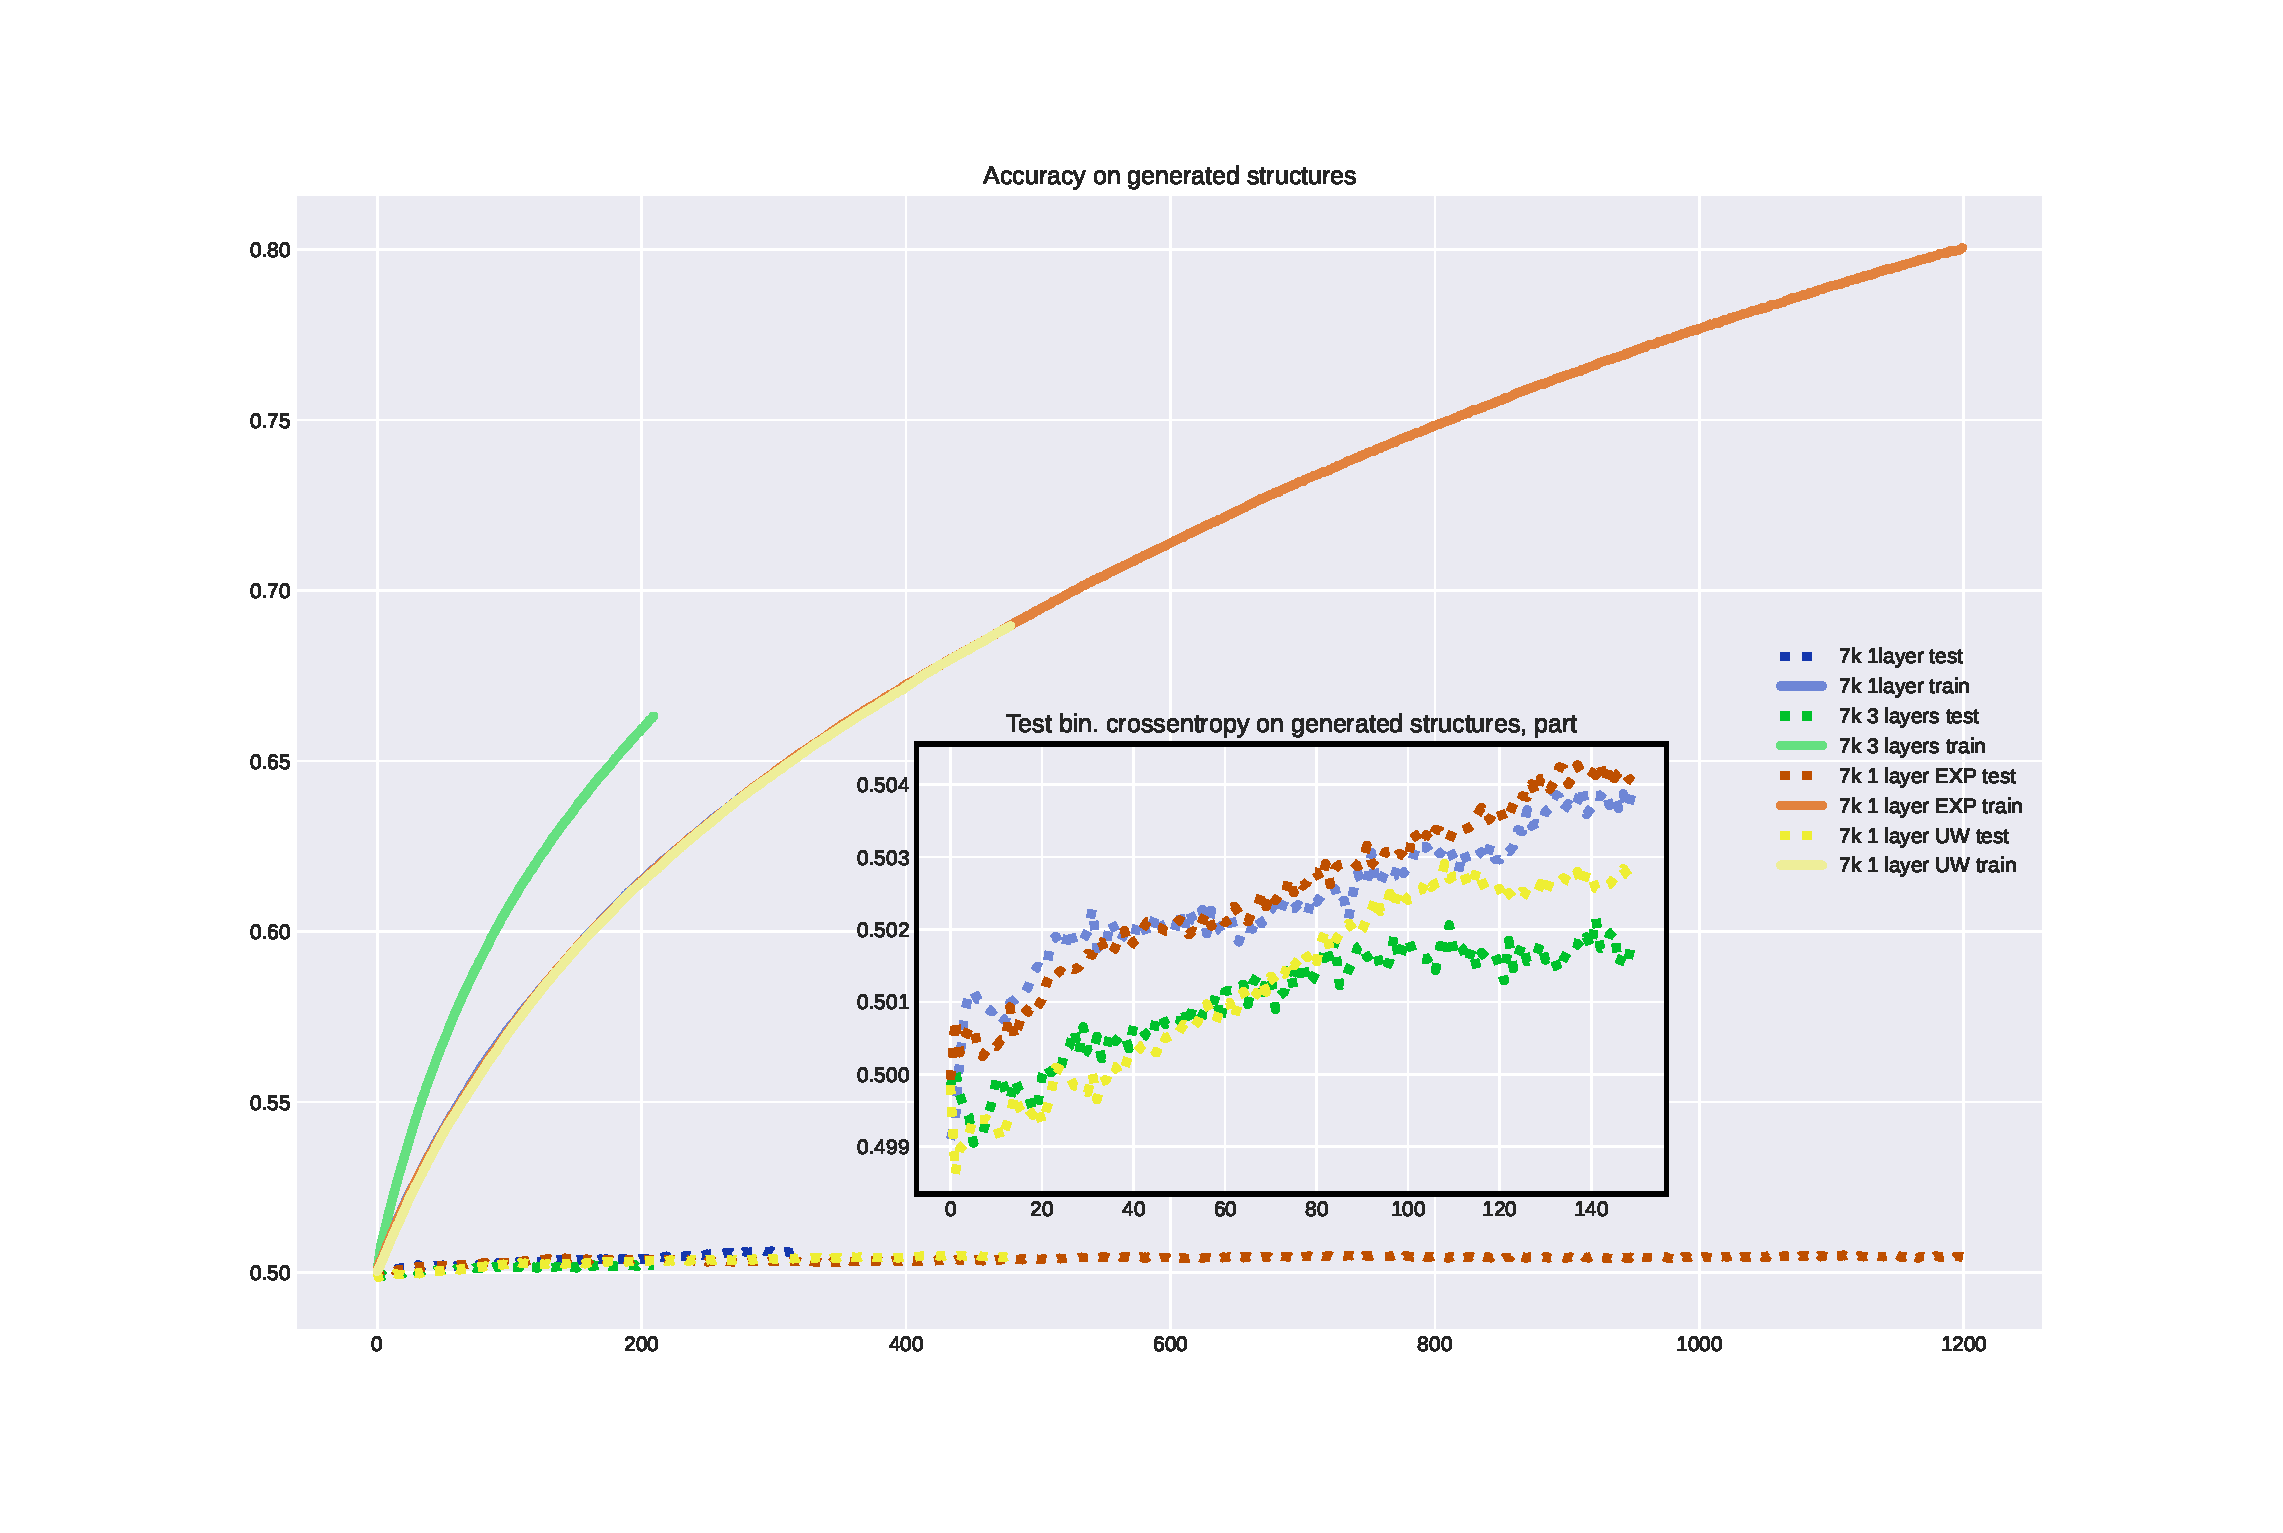
\includegraphics[width=\linewidth]{imgs/acc-7k.eps}
  \caption{Точность простой полносвязной нейросети в процессе обучения}\label{fig:acc_7k}
\endminipage\hfill
\minipage{0.5\textwidth}%
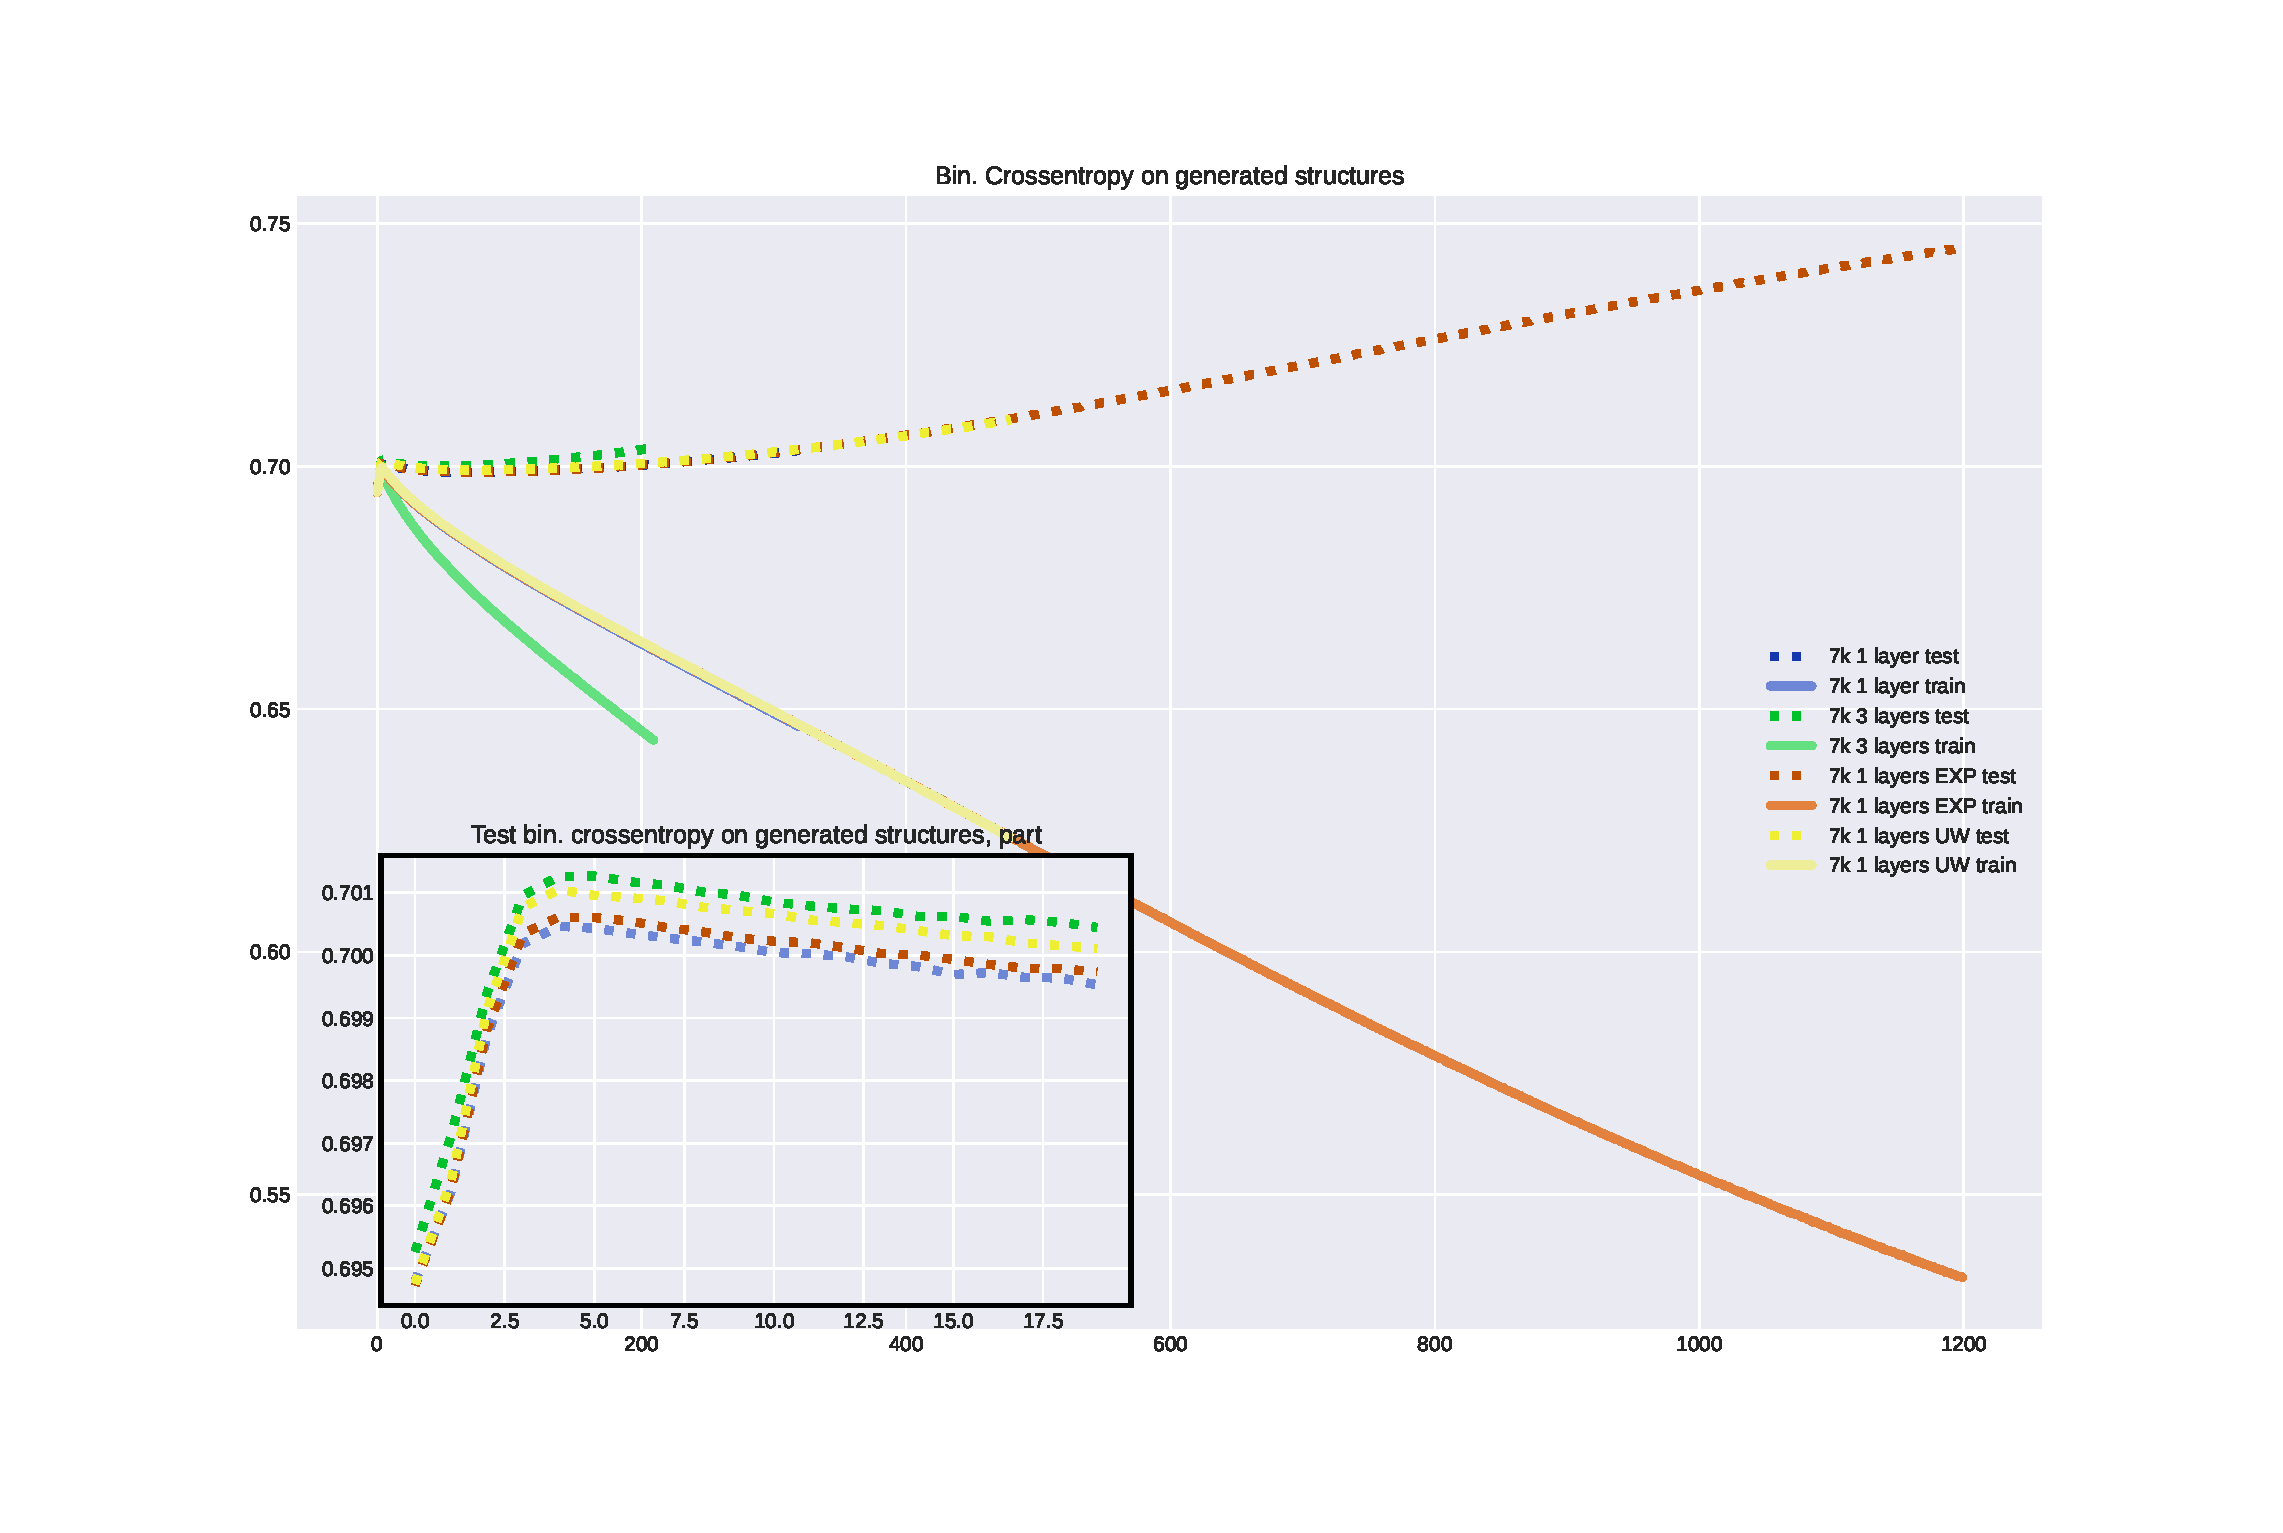
\includegraphics[width=\linewidth]{imgs/loss-7k.eps}
  \caption{Функция потерь простой полносвязной нейросети в процессе обучения}\label{fig:loss_7k}
\endminipage
\end{figure}

Из этого был сделан вывод о том, что данных для обучения модели недостаточно, и необходимо увеличить датасет. Другим возможным путем решения проблемы переобучения является снижение запоминающей способности сети путем добавления дропаутов, регуляризации, снижения количества нейронов в скрытых слоях сети и числа скрытых слоев.

\subsection{Обучение нейронной сети на данных CCDC}

Было проведено обучение нейросети на данных CCDC с разными гиперпараметрами и размером датасета. Для ускорения расчетов в части экспериментов были отброшены отражения с наибольшими индексами $h,k,l$, оставлены лишь удовлетворяющие условию $h^2+k^2+l^2<50$. После отбрасывания в каждом файле осталось по 709 отражений. Получены следующие результаты:

Для части датасета в 50 тысяч файлов, с отброшенными дальними отражениями была проведена проверка относительного качества обучения двух моделей: с одним внутренним слоем из 709 нейронов и с тремя внутренними слоями из 709 нейронов. Графики обучения (рис. \ref{fig:acc_50k}, \ref{fig:loss_50k}) демонстрируют сильное переобучение в обоих случаях, однако в случае с одним слоем оно менее выражено. Это говорит о том, что обе модели имеют избыточную запоминающую способность.

\begin{figure}[!h]
\minipage{0.5\textwidth}
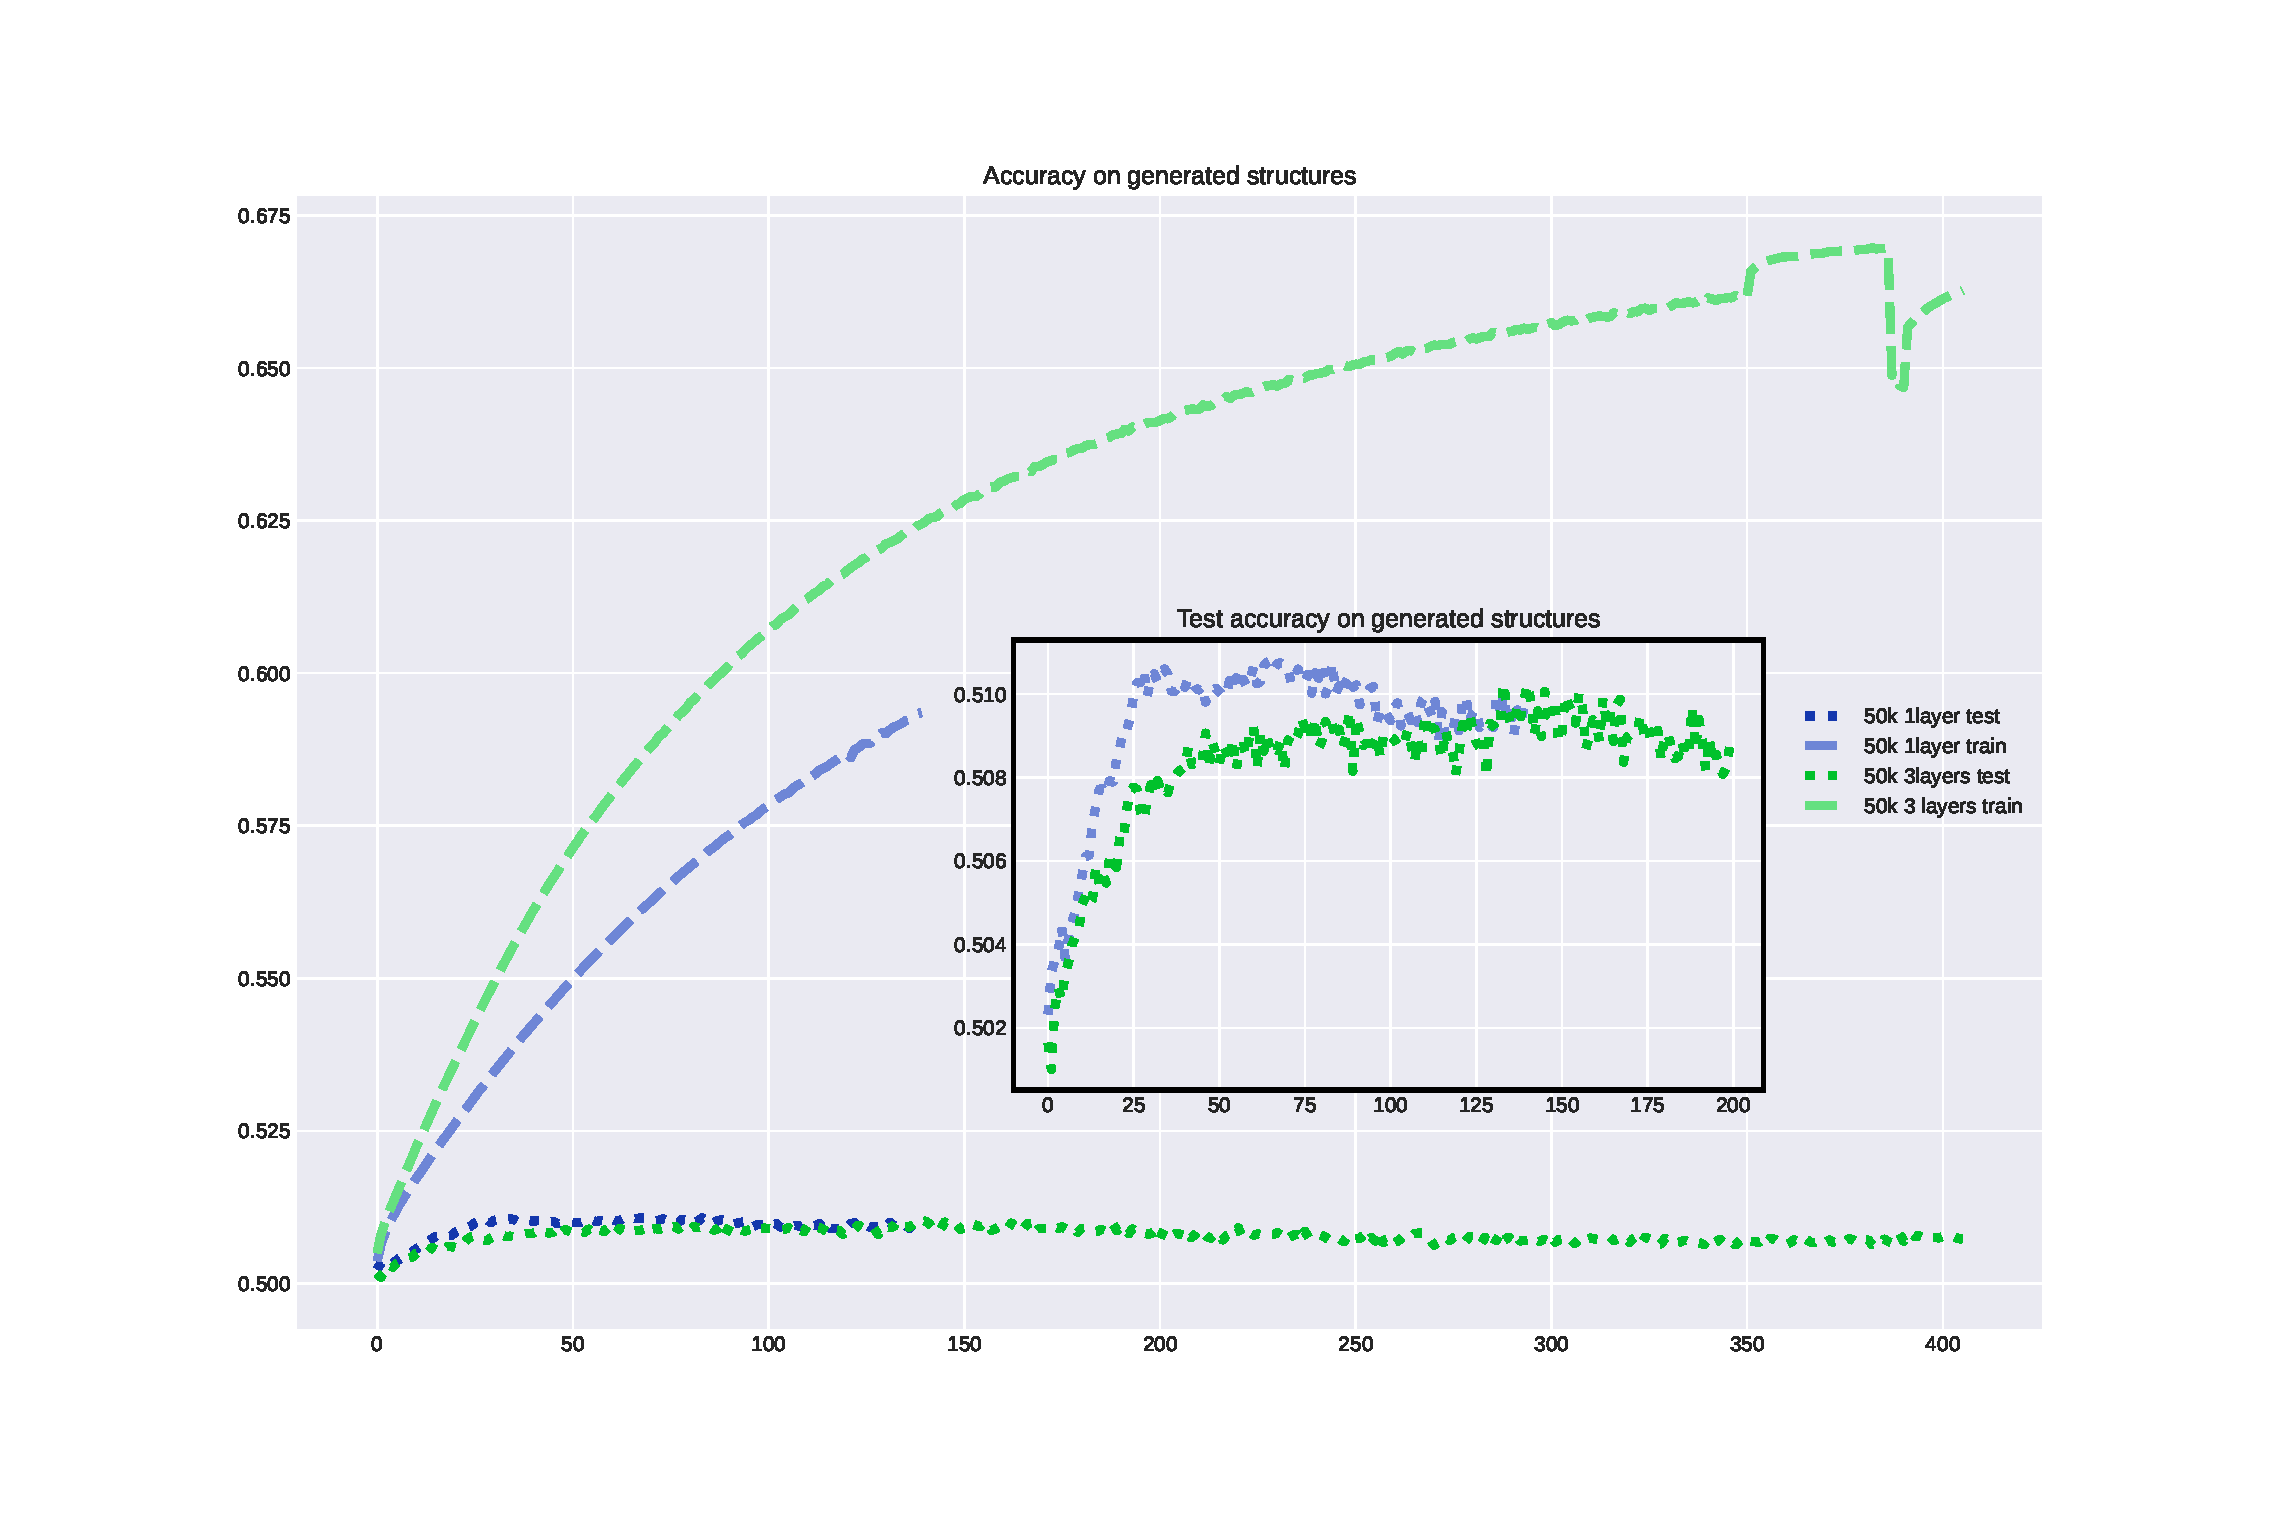
\includegraphics[width=\linewidth]{imgs/acc-50k.eps}
  \caption{Точность нейросети с одним и тремя слоями}\label{fig:acc_50k}
\endminipage\hfill
\minipage{0.5\textwidth}%
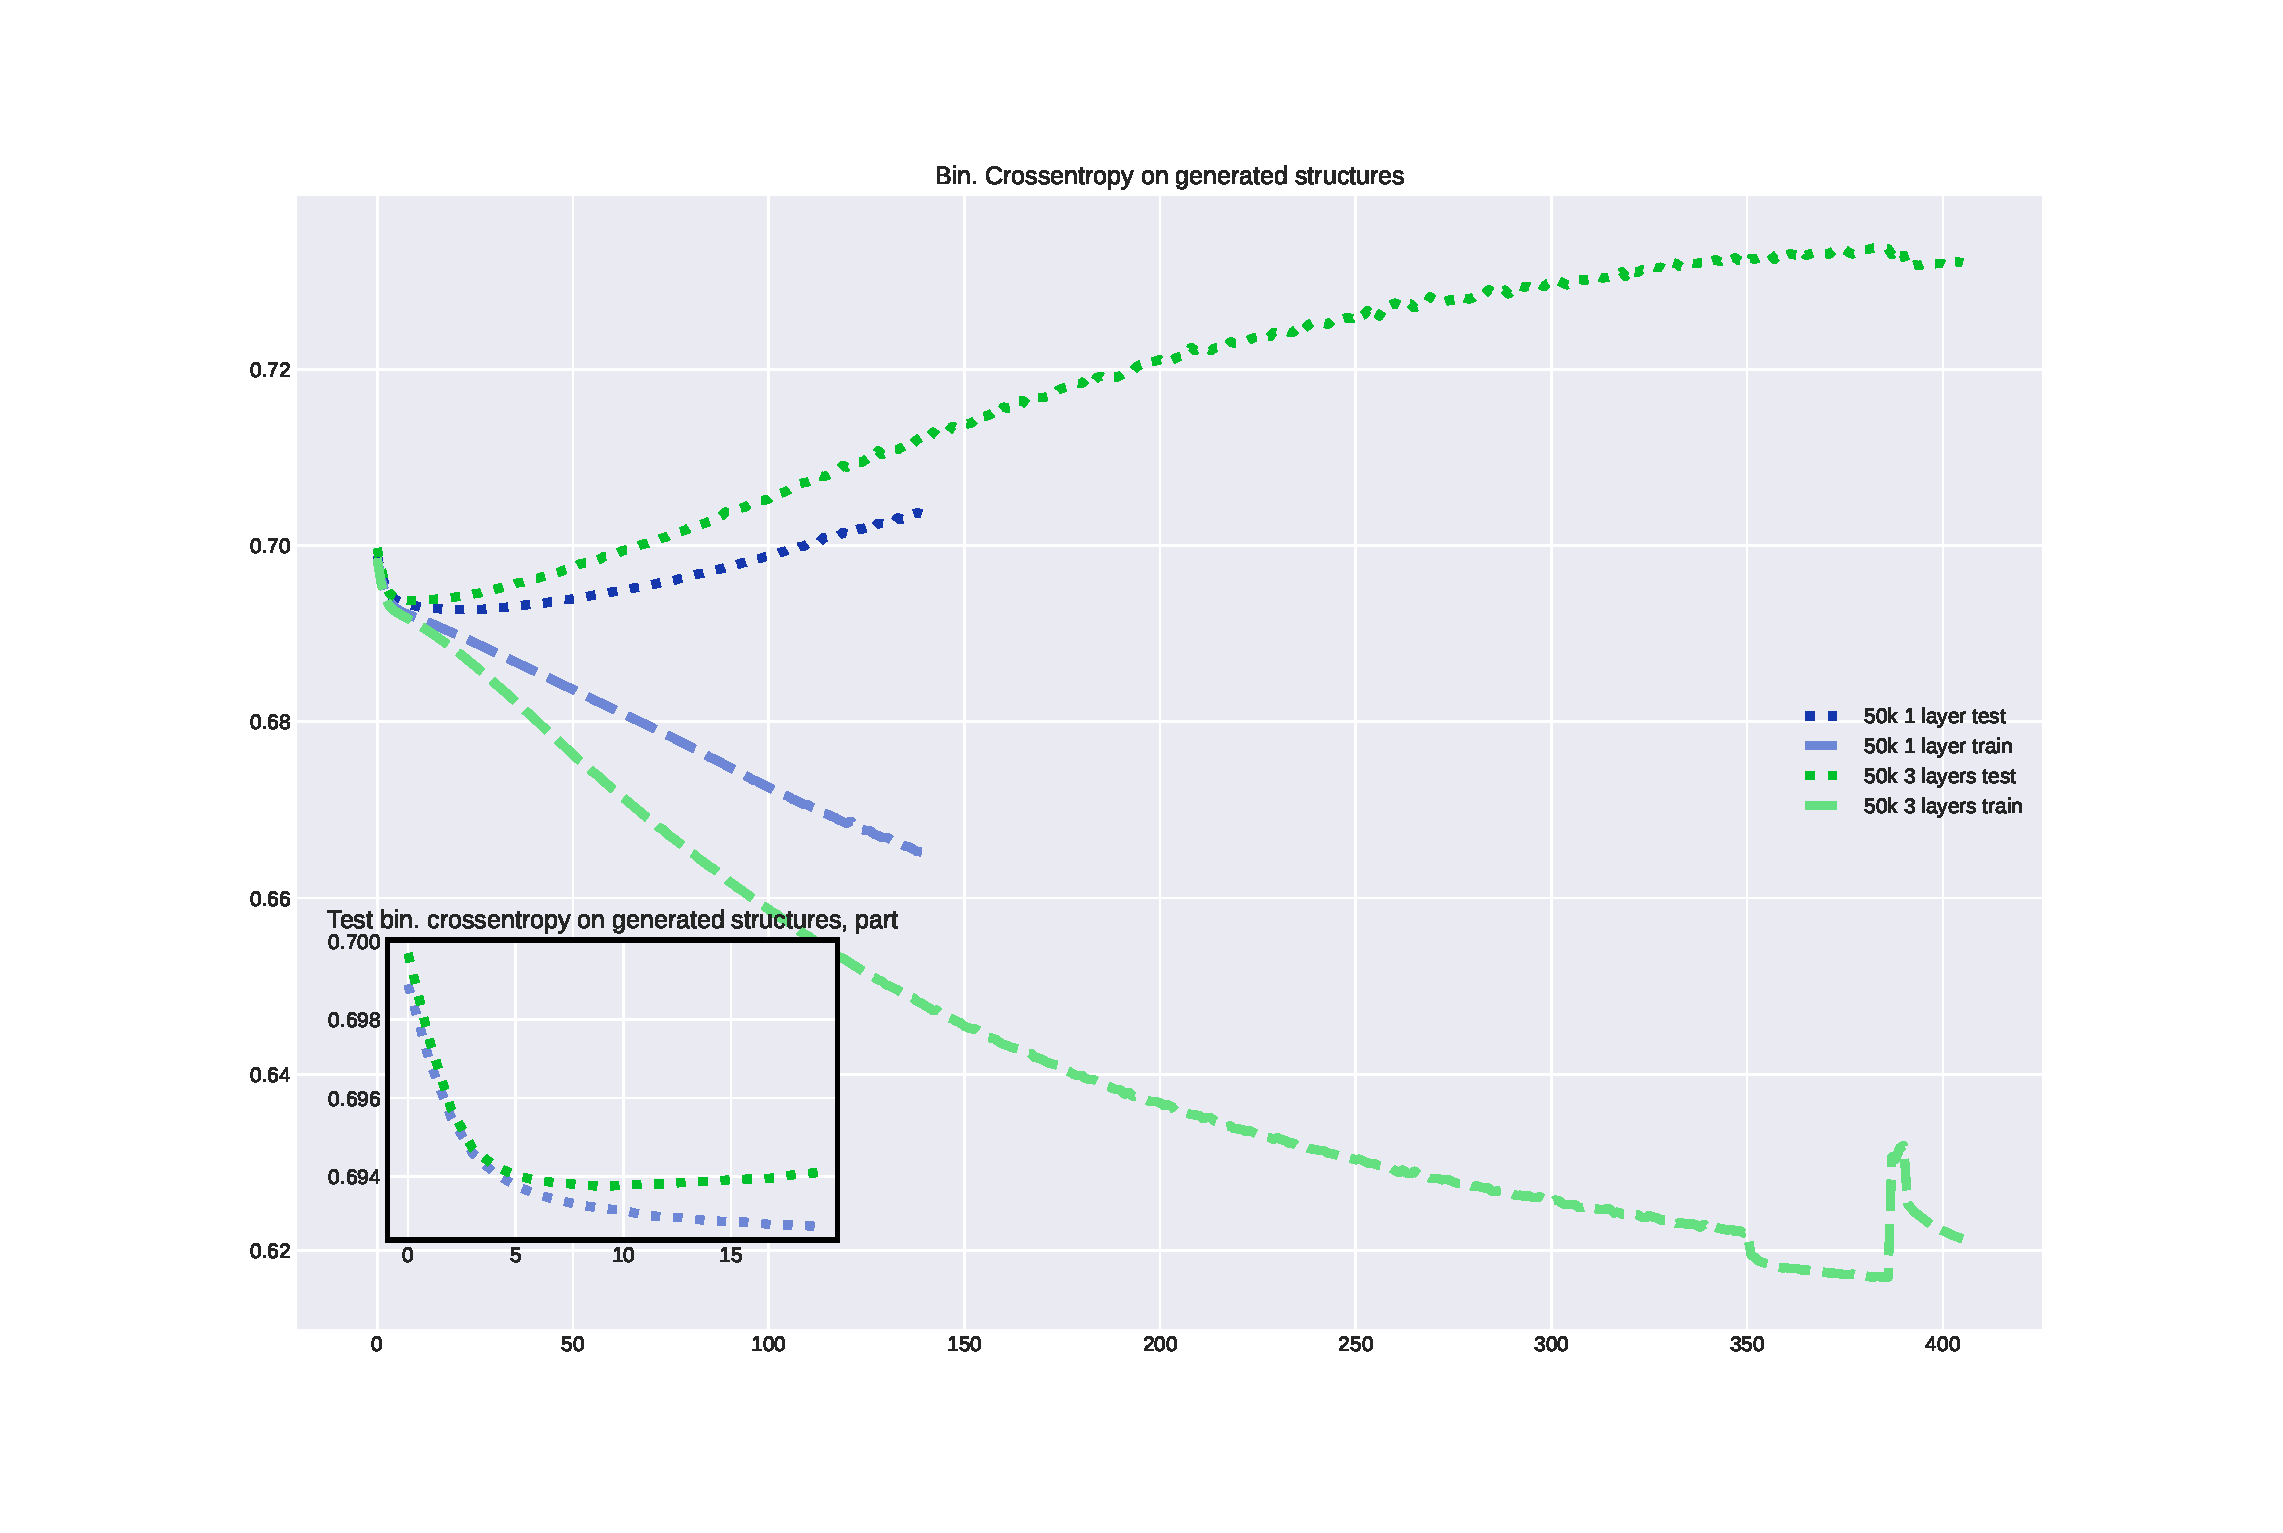
\includegraphics[width=\linewidth]{imgs/loss-50k.eps}
  \caption{Функция ошибки нейросети с одним и тремя слоями}\label{fig:loss_50k}
\endminipage
\end{figure}

Был проверена зависимость качества обучения от размера датасета. Было проведено обучение на разном количестве данных - 7000 файлов, 50 тысяч файлов, 150 тысяч файлов, с отбросом дальних отражений. На графиках обучения(рис. \ref{fig:acc_1l_ndata}, \ref{fig:loss_1l_ndata}) видно что больший размер датасета приводит к меньшему переобучению, %ну вот кто бы мог подумать?..

\begin{figure}[!h]
\minipage{0.5\textwidth}
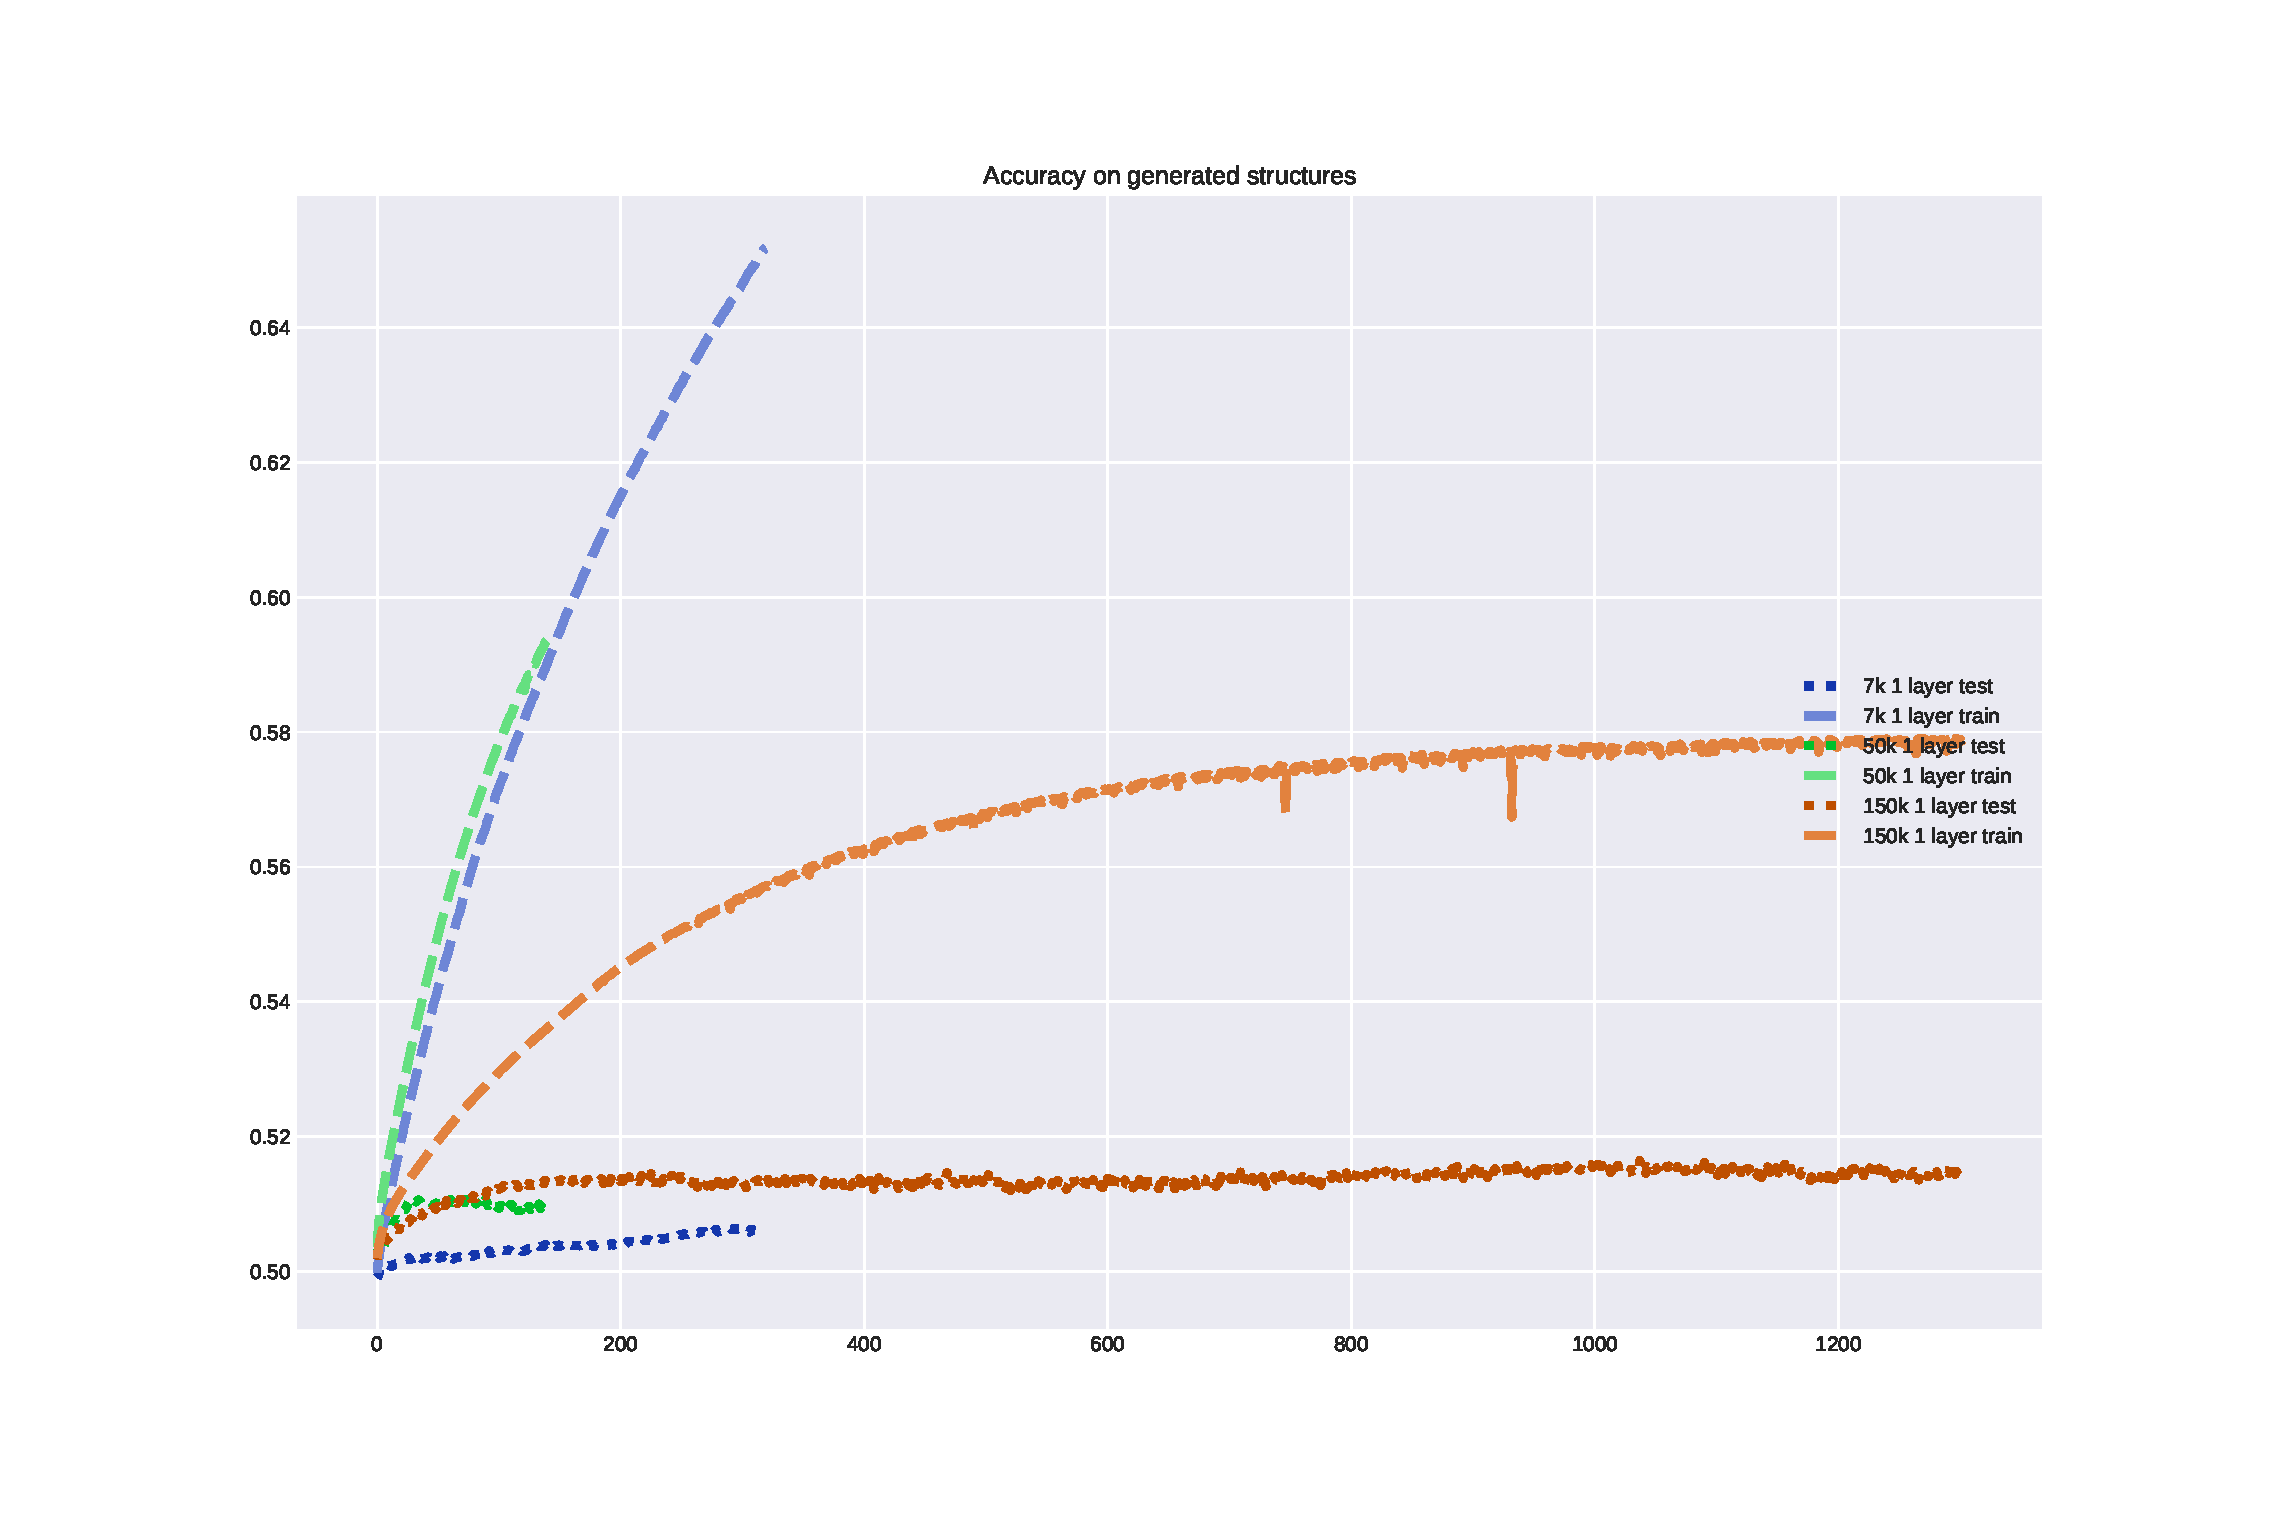
\includegraphics[width=\linewidth]{imgs/acc-1l_ndata.eps}
  \caption{Точность нейросети с одним слоем на разном количестве данных}\label{fig:acc_1l_ndata}
\endminipage\hfill
\minipage{0.5\textwidth}%
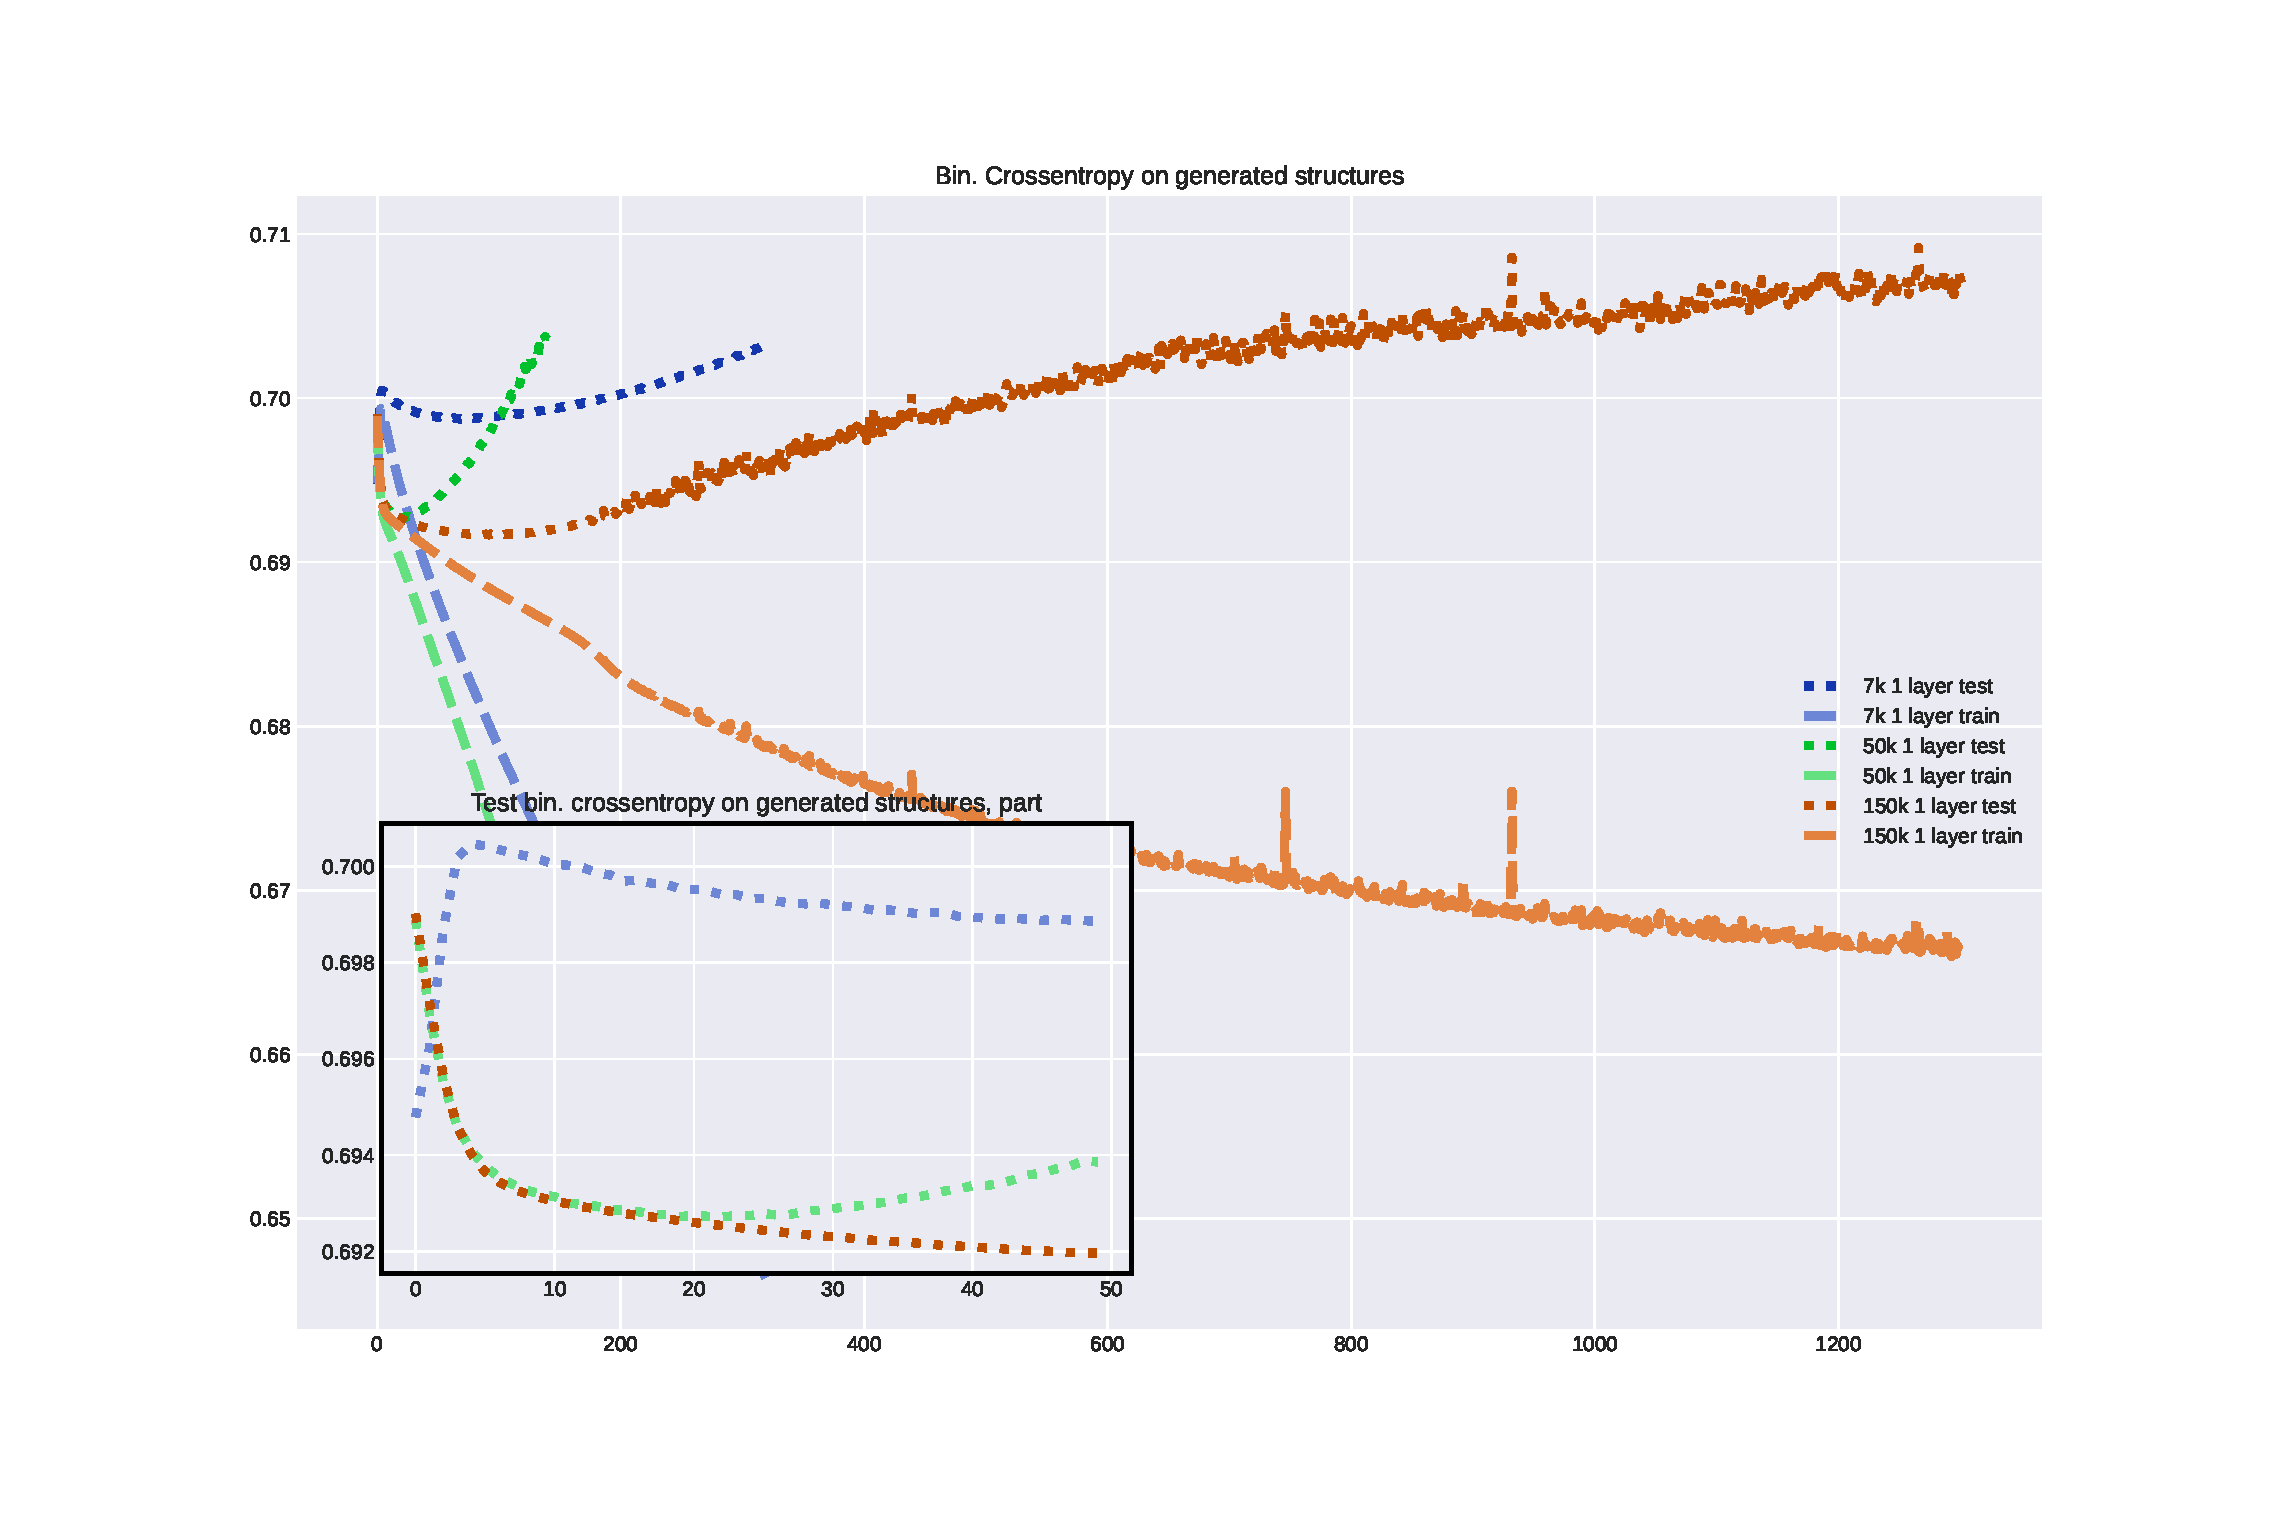
\includegraphics[width=\linewidth]{imgs/loss-1l_ndata.eps}
  \caption{Функция ошибки нейросети с одним слоем на разном количестве данных}\label{fig:loss_1l_ndata}
\endminipage
\end{figure}


Тот же результат был получен и при обучении нейросети из 3 слоев. Также было проведено обучение на 7000, 50 тысячах и 150 тысячах фалов. Заметно переобучение, оно уменьшается при увеличении размеров датасета, что можно видеть по рисункам \ref{fig:acc_3l_ndata}, \ref{fig:loss_3l_ndata}.
\begin{figure}[!h]
\minipage{0.5\textwidth}
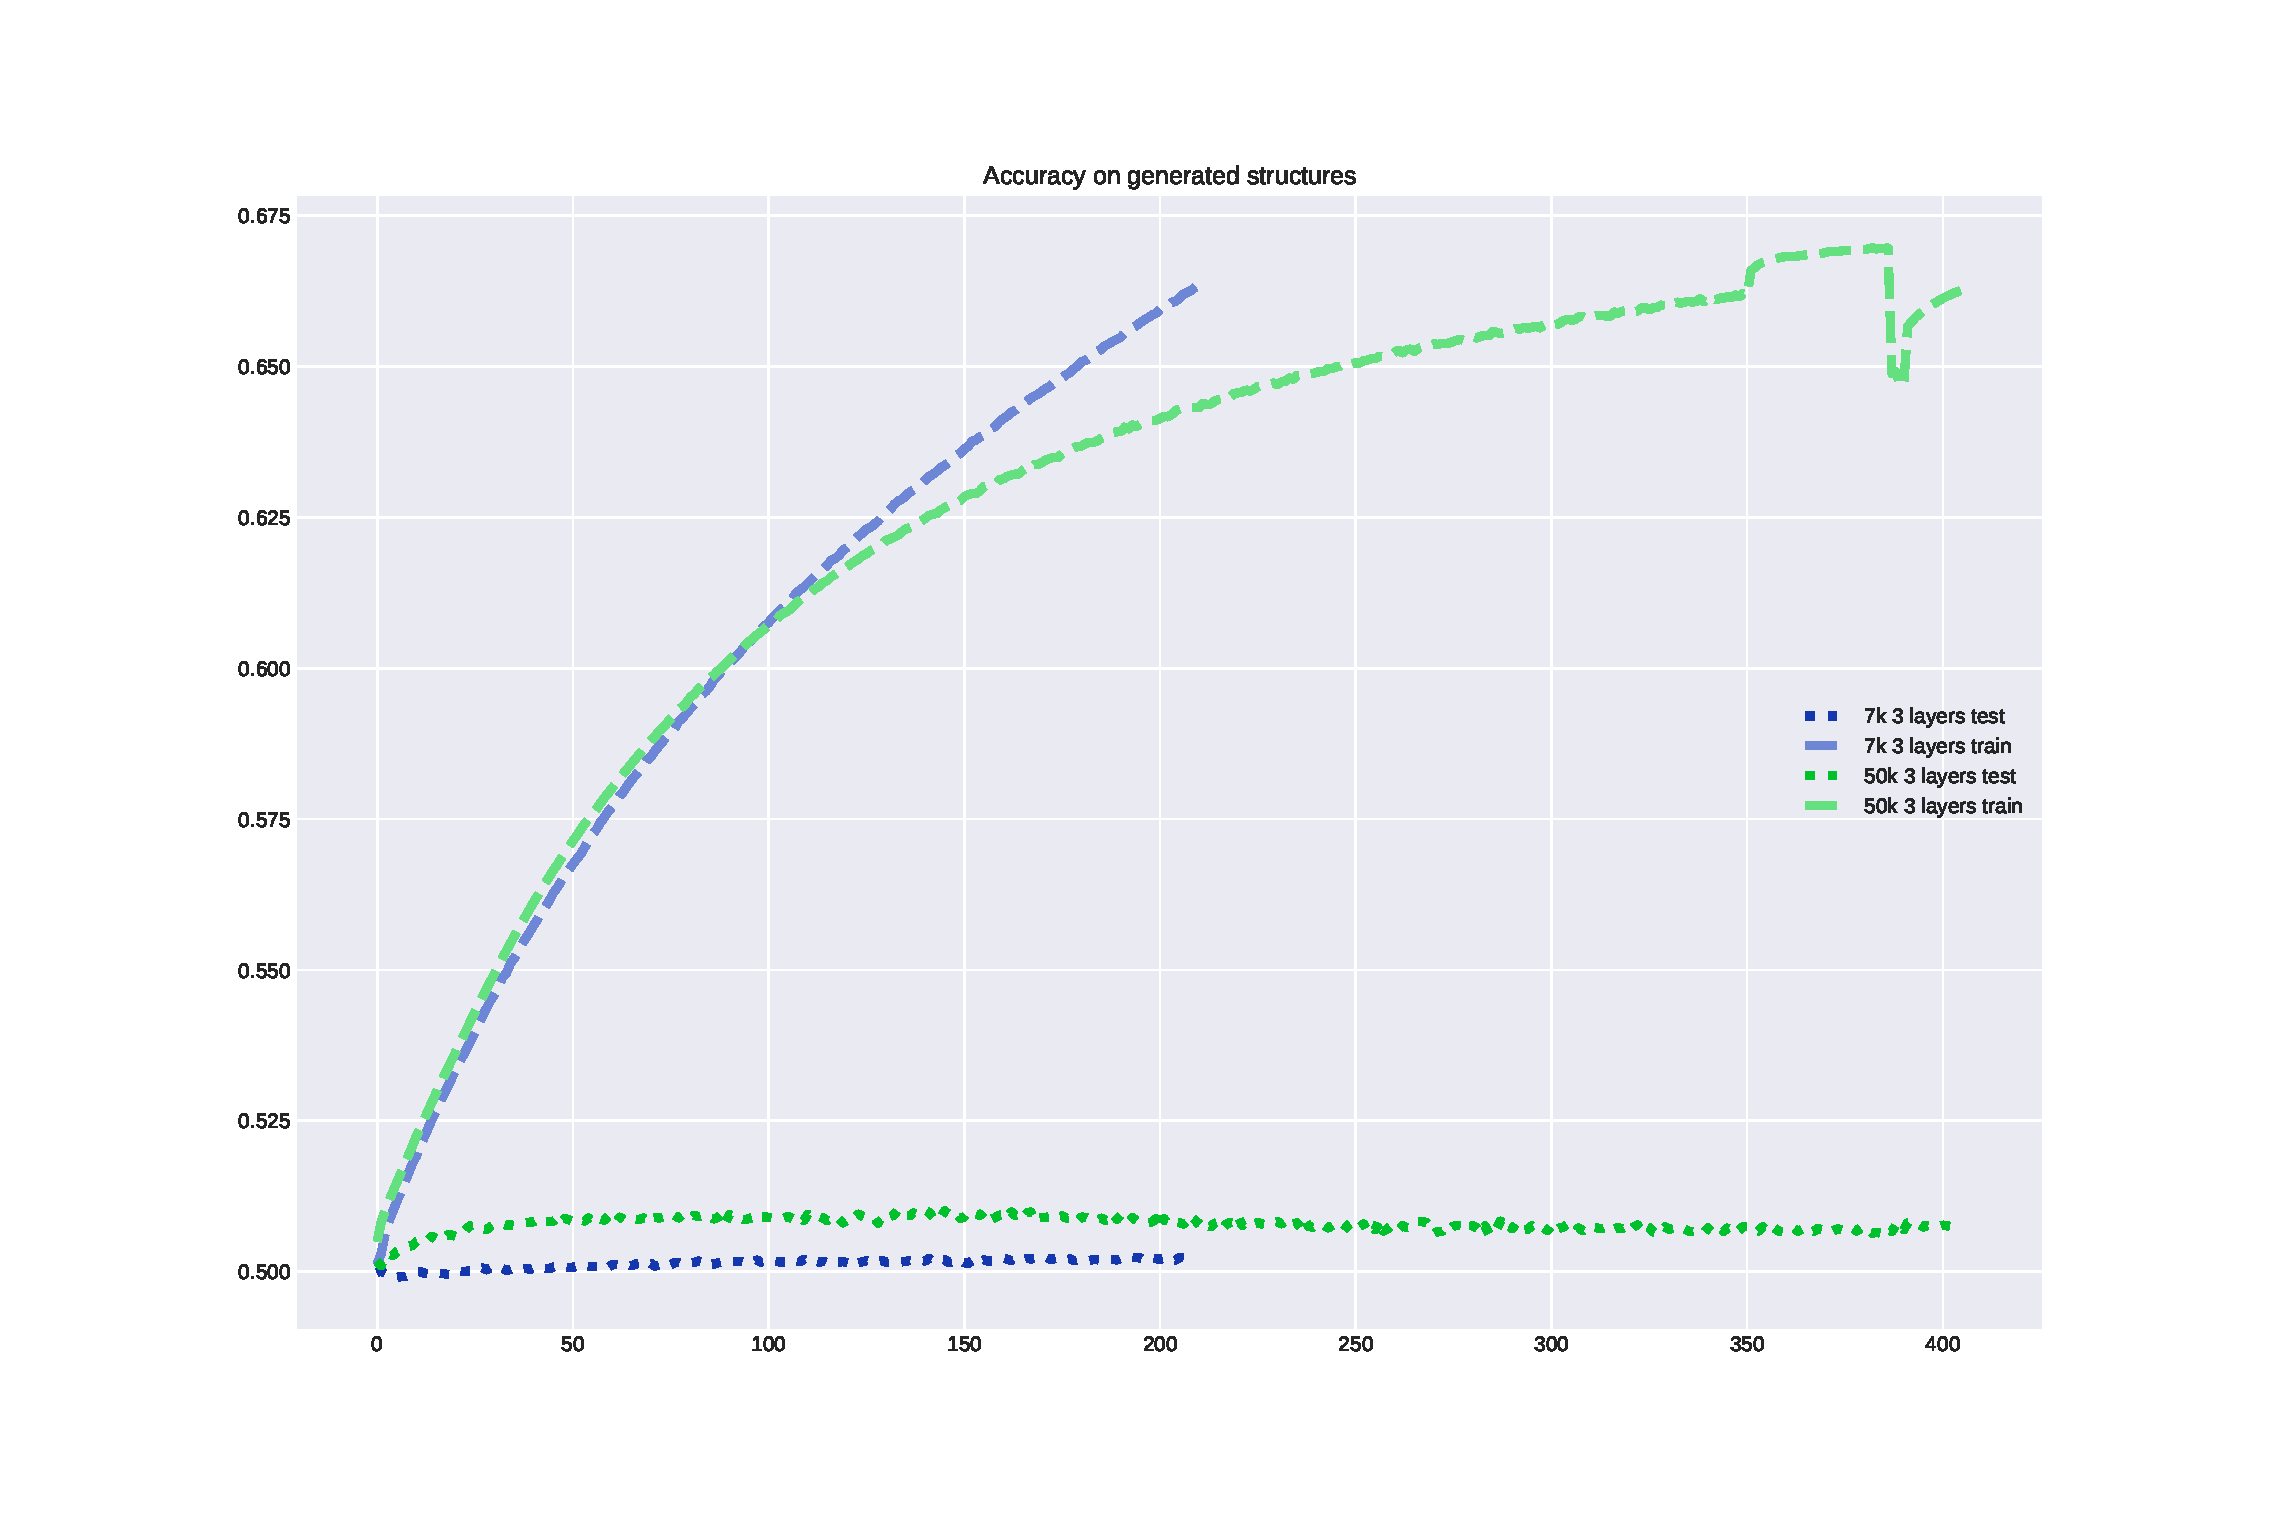
\includegraphics[width=\linewidth]{imgs/acc-3l_ndata.eps}
  \caption{Точность нейросети с одним слоем на разном количестве данных}\label{fig:acc_3l_ndata}
\endminipage\hfill
\minipage{0.5\textwidth}%
\includegraphics[width=\linewidth]{imgs/loss-3l_ndata.eps}
  \caption{Функция ошибки нейросети с одним слоем на разном количестве данных}\label{fig:loss_3l_ndata}
\endminipage
\end{figure}

\subsection{Зависимость качества обучения от типа весов}

Функцю ошибки, на основе которой проводится обучение модели, можно взвесить по какой-либо характеристике, как и метрику. Была исследована зависимость качества обучения от весов применемой в модели метрики. Результаты представлены на рис. \ref{fig:acc_weight}, \ref{fig:loss_weight}

Лучший результат дает обучнение с функцией ошибки взвешенной по интенсивности отражений. Взвешивание по экспоненте от интенсивности отражений, а также отсутствие взвешивания(равный вес всех отражений) дали незначительно худшие реультаты. 

\begin{figure}[!h]
\minipage{0.5\textwidth}
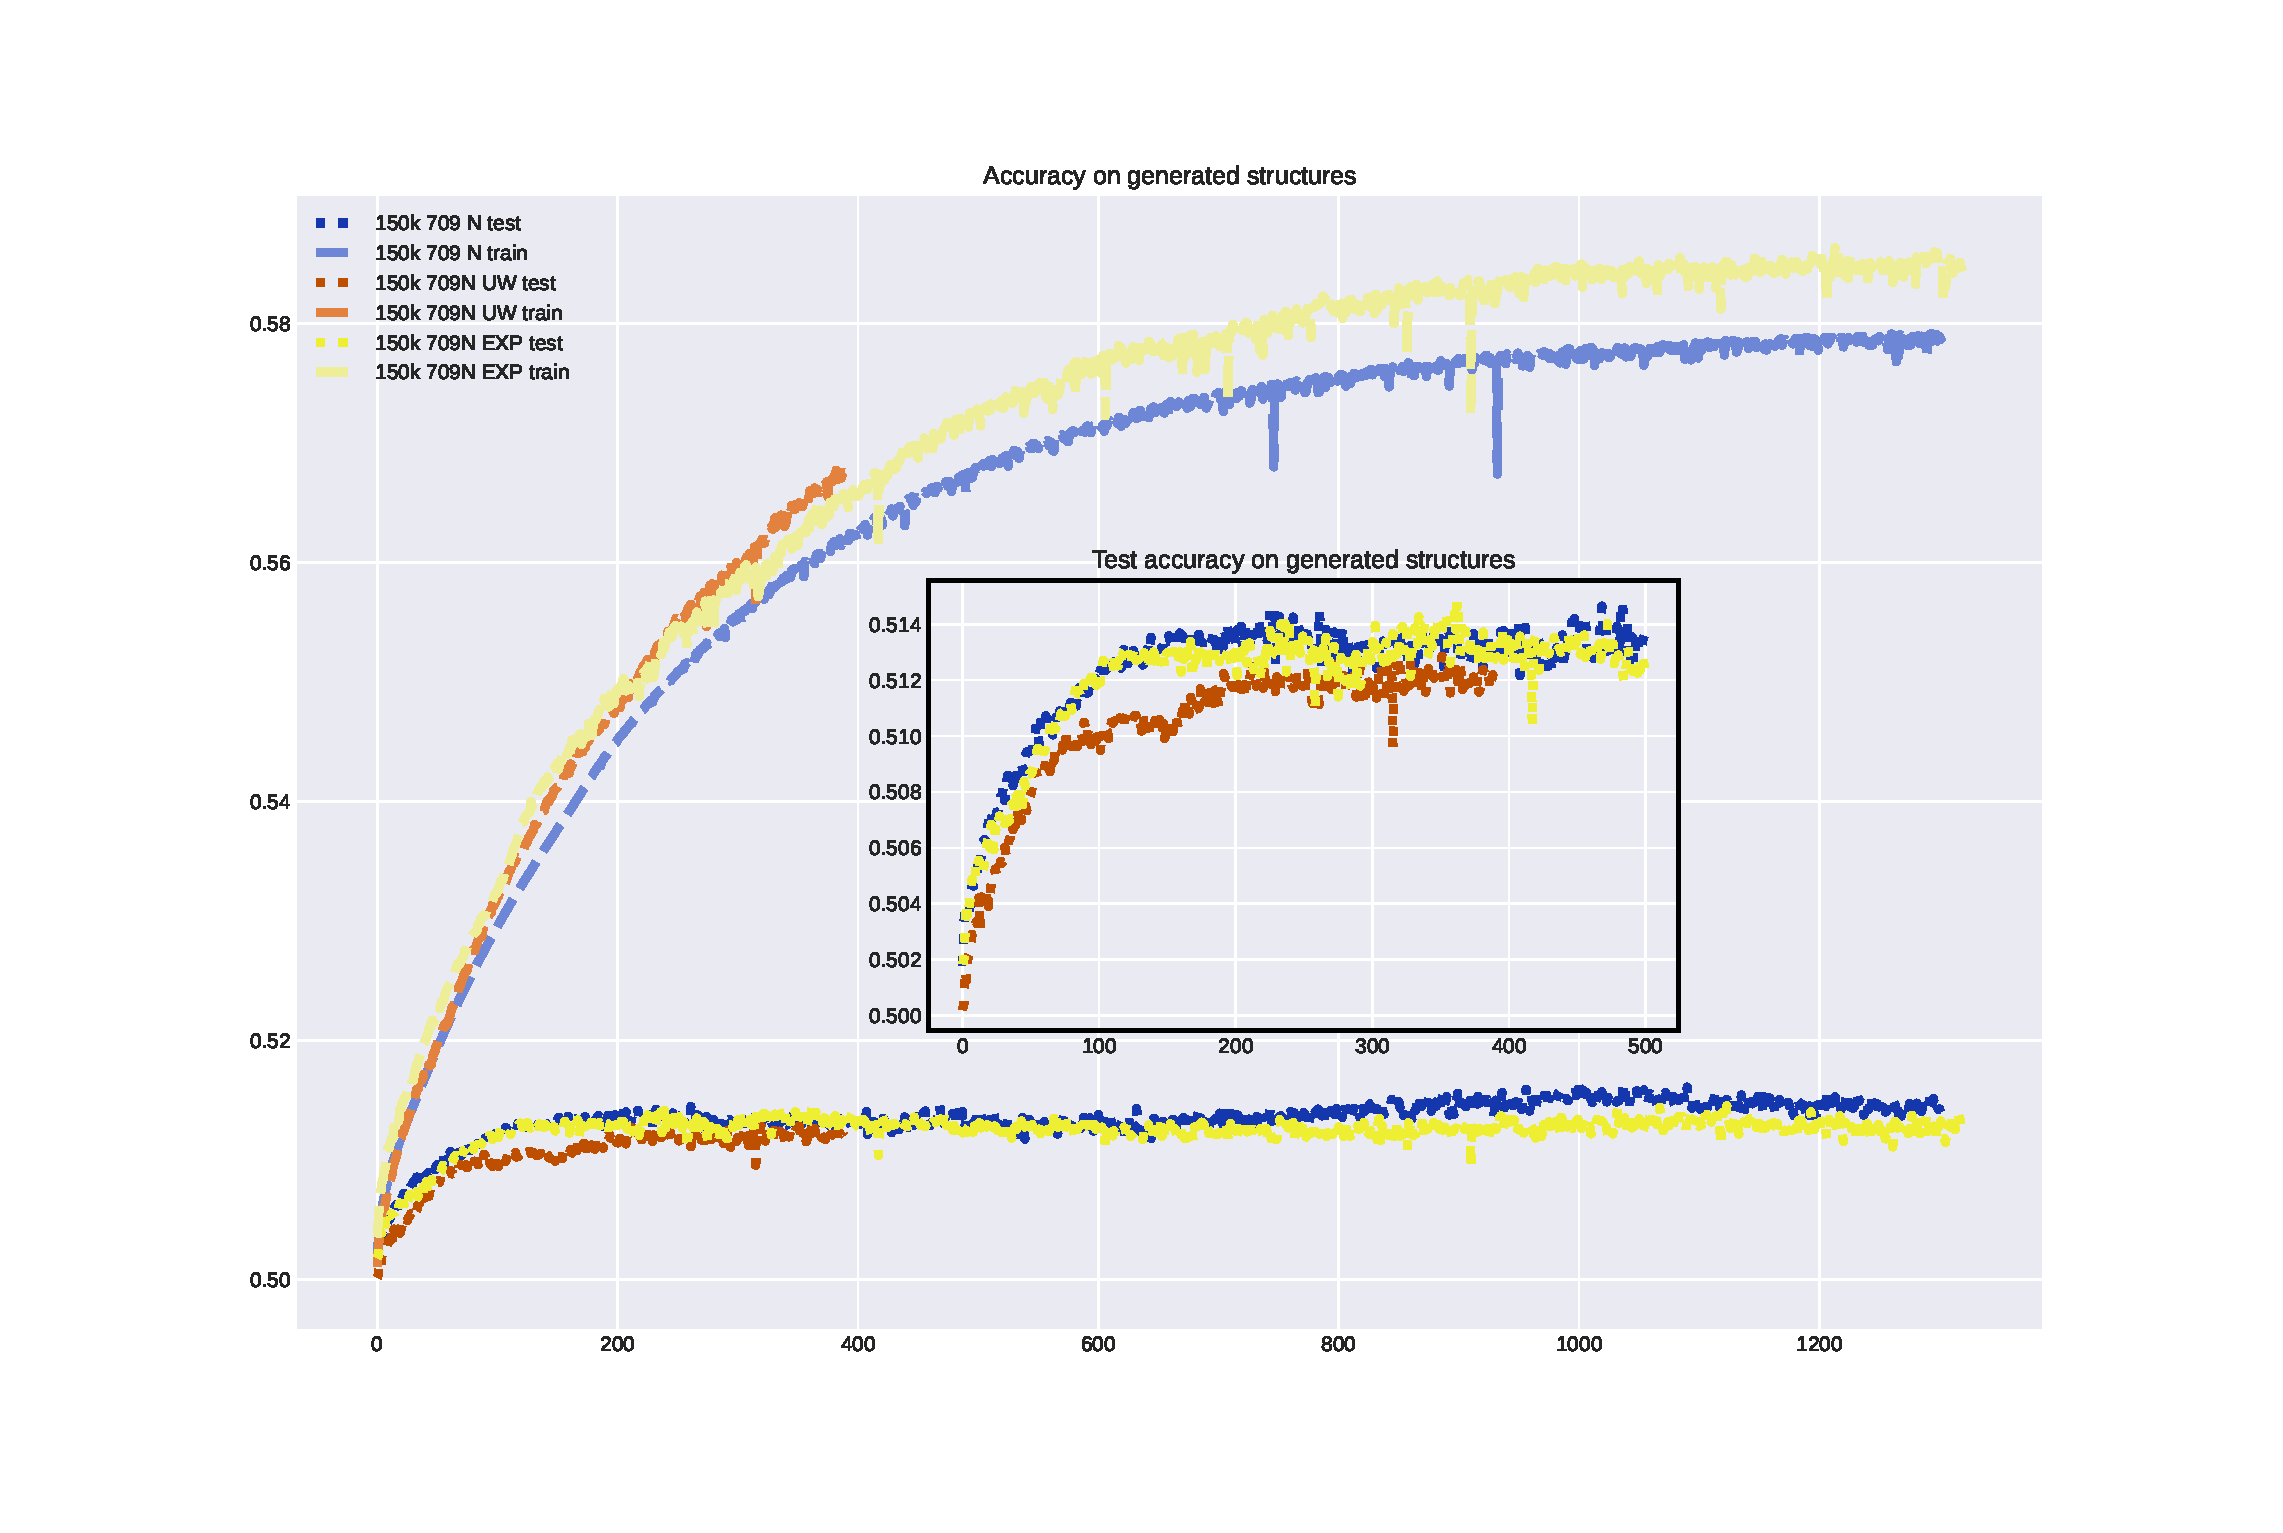
\includegraphics[width=\linewidth]{imgs/acc-weight.eps}
  \caption{Точность нейросети в зависимости от весов функции ошибки}\label{fig:acc_weight}
\endminipage\hfill
\minipage{0.5\textwidth}%
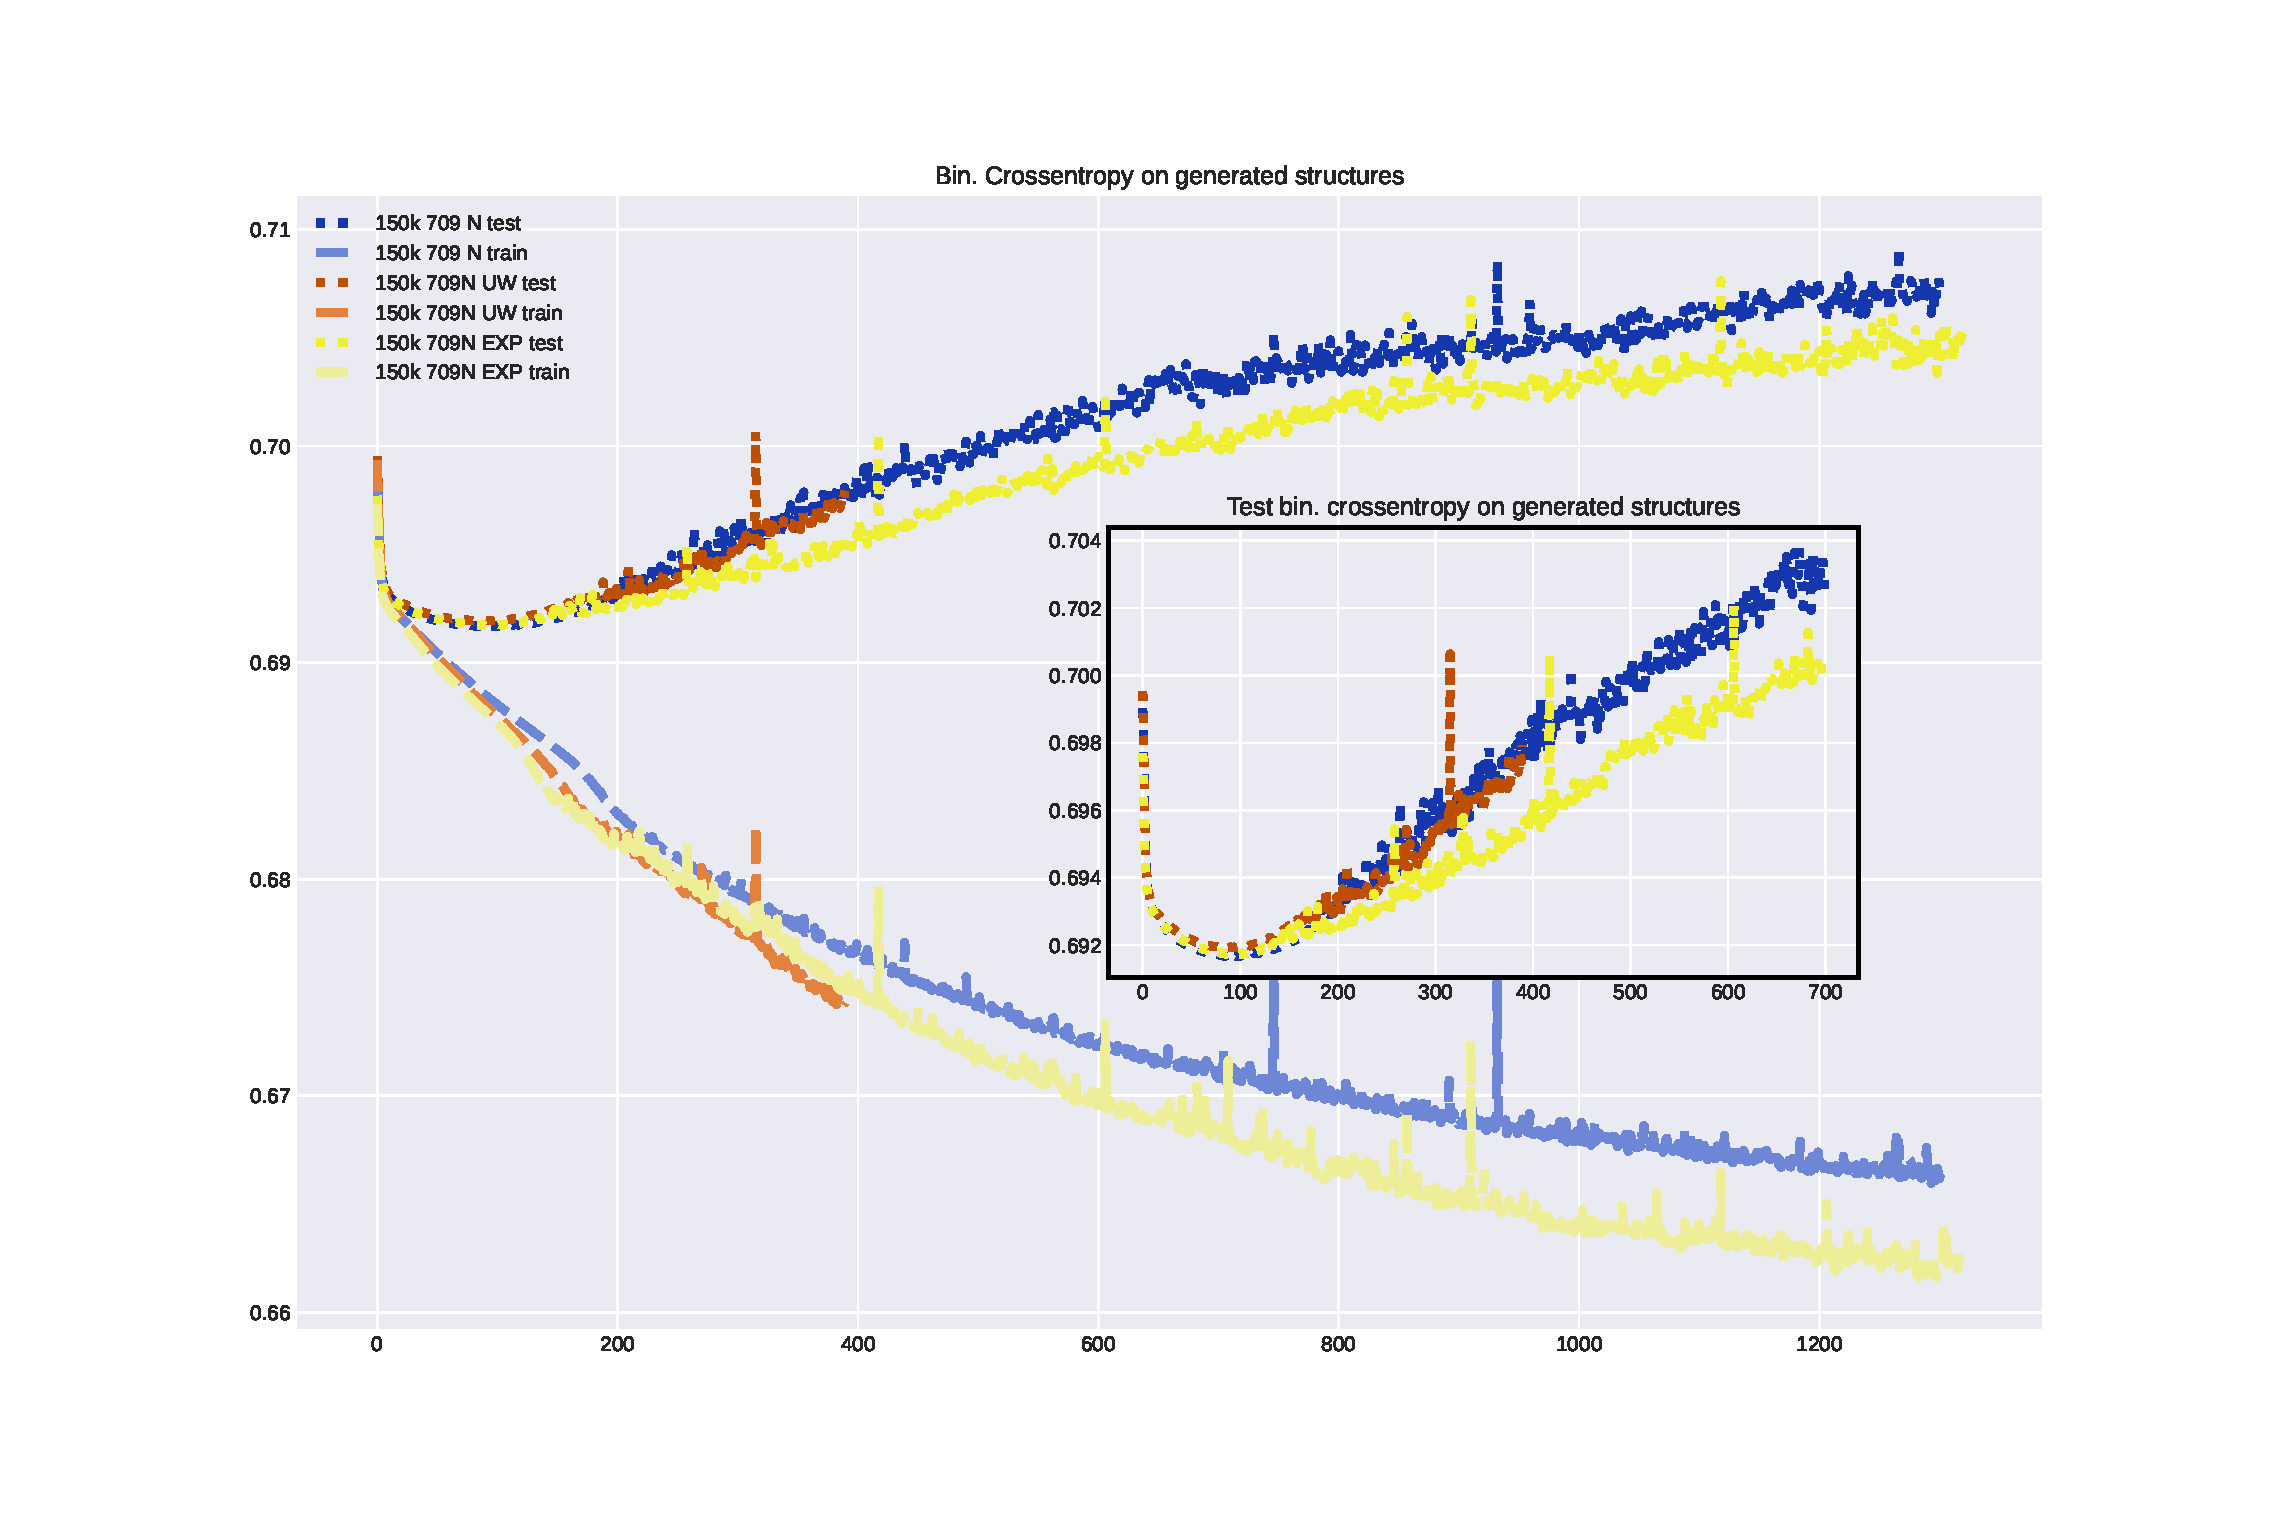
\includegraphics[width=\linewidth]{imgs/loss-weight.eps}
  \caption{Функция ошибки нейросети в зависимости от весов функции ошибки}\label{fig:loss_weight}
\endminipage
\end{figure}



\begin{figure}[h!tp]
\centering
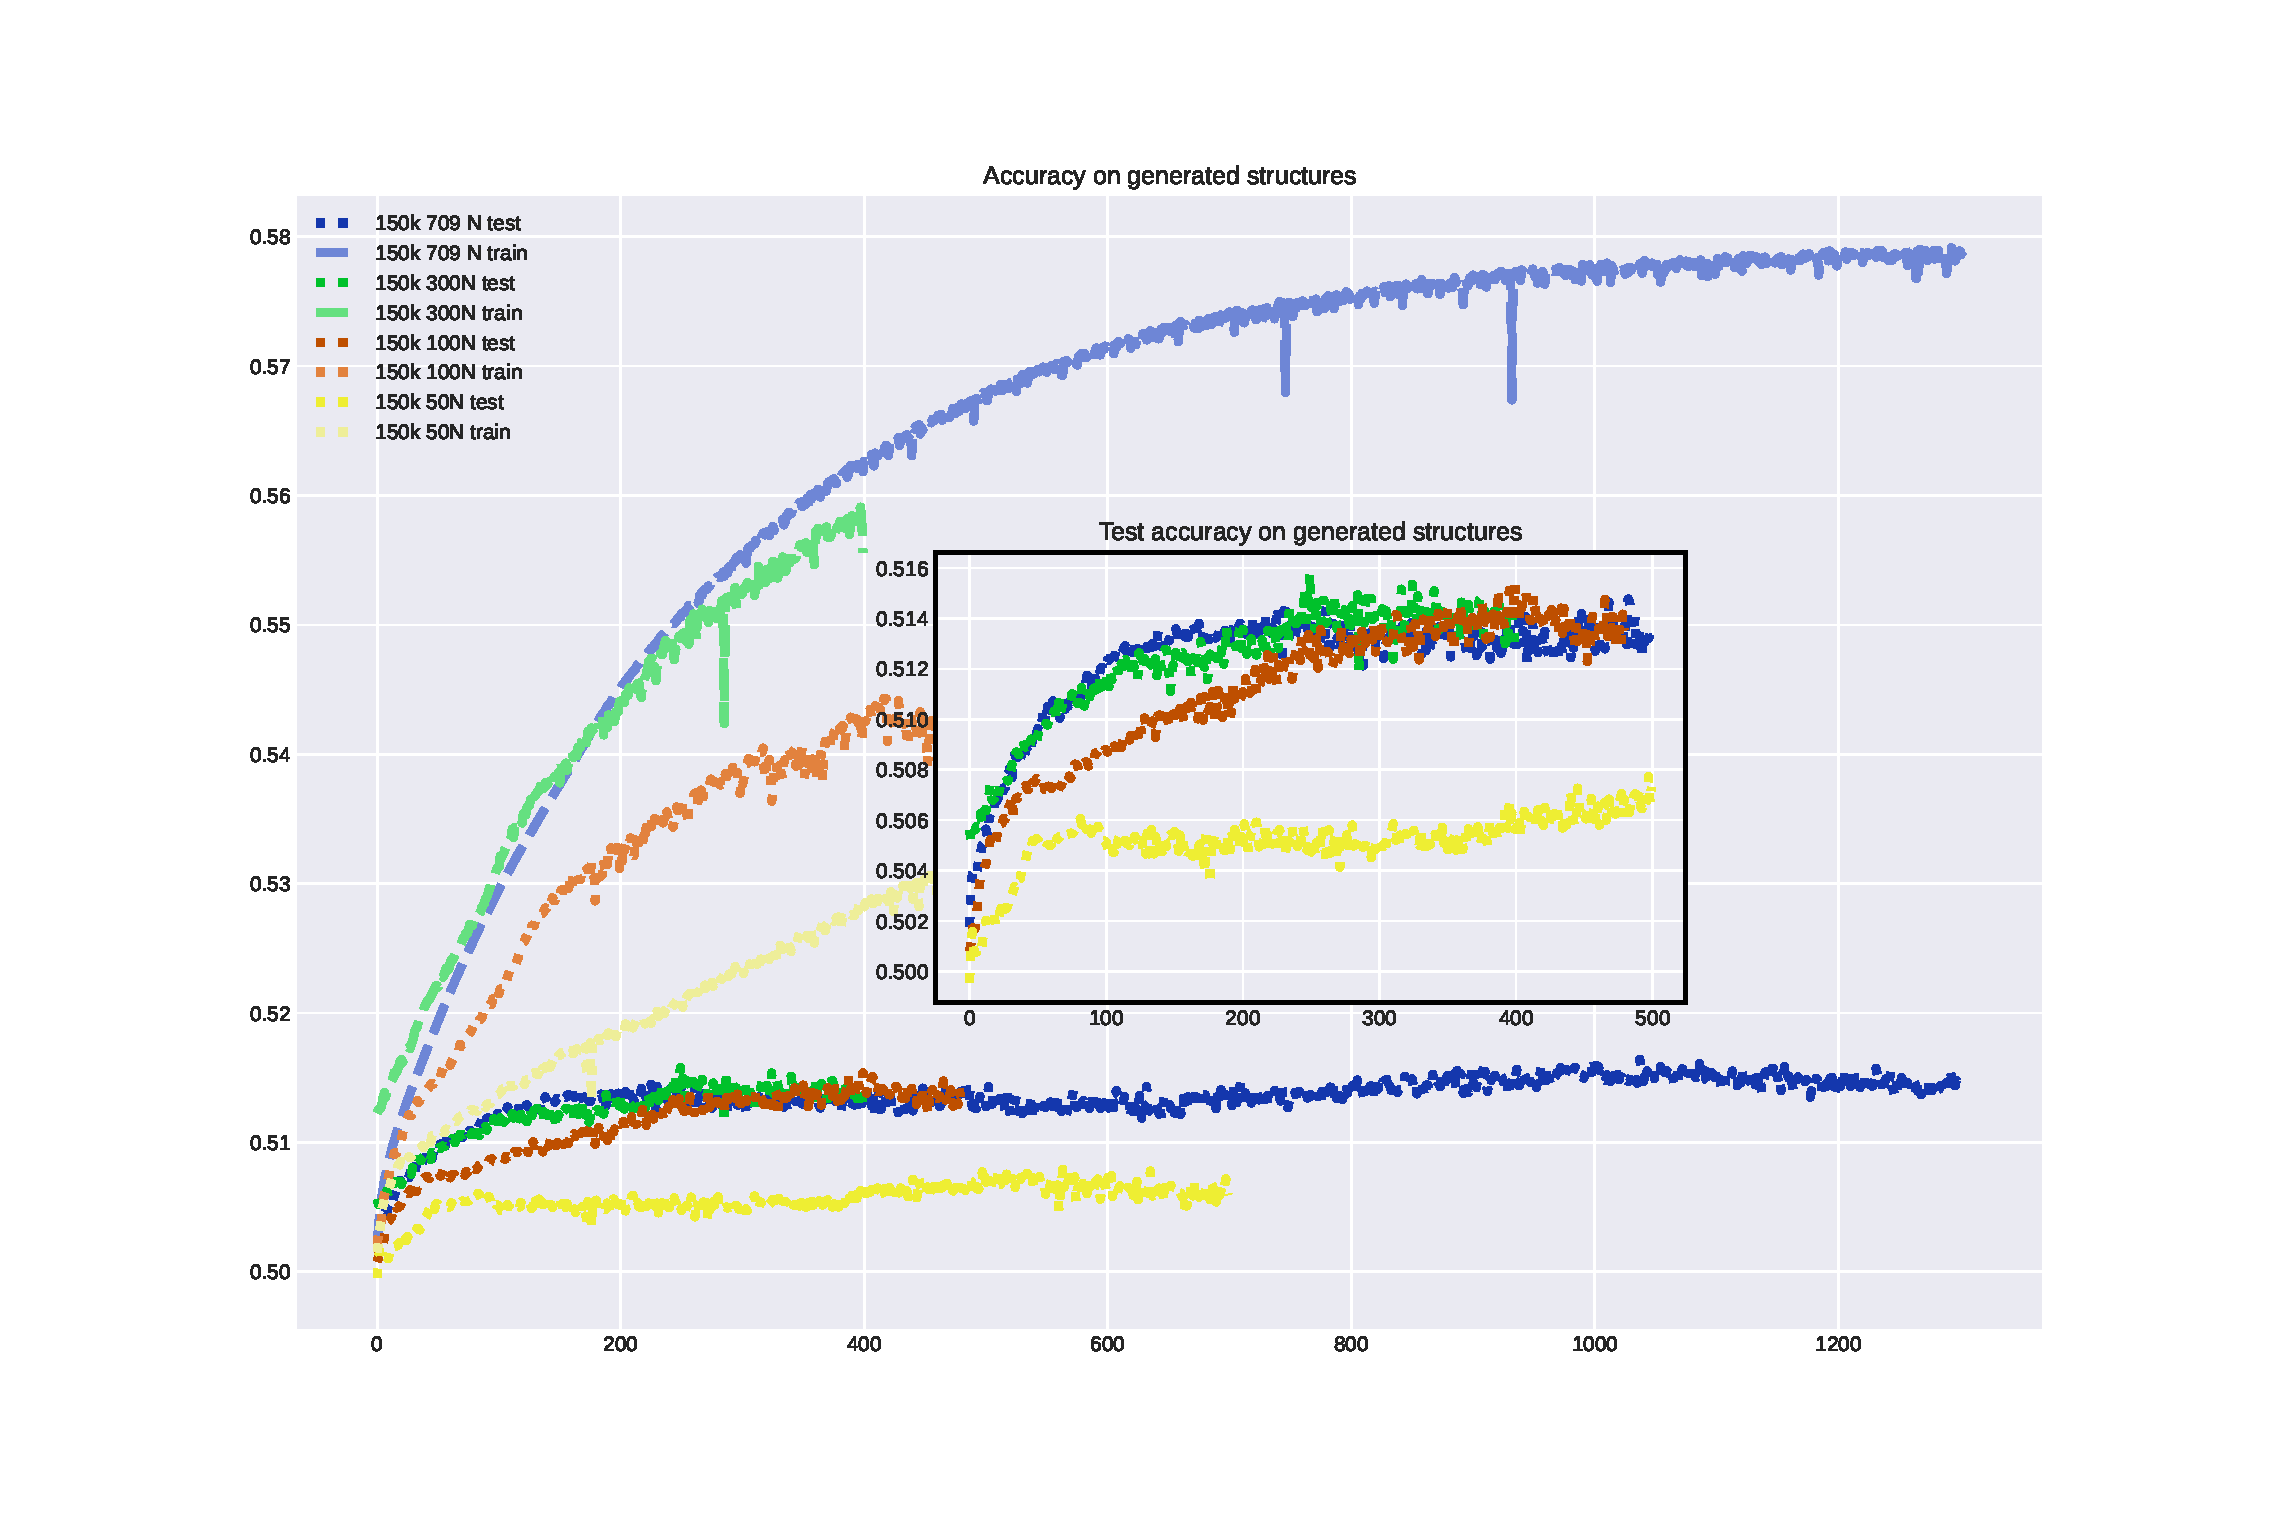
\includegraphics[scale=.500]{imgs/acc-lsize.eps}
\caption{}
\label{}
\end{figure}

\begin{figure}[h!tp]
\centering
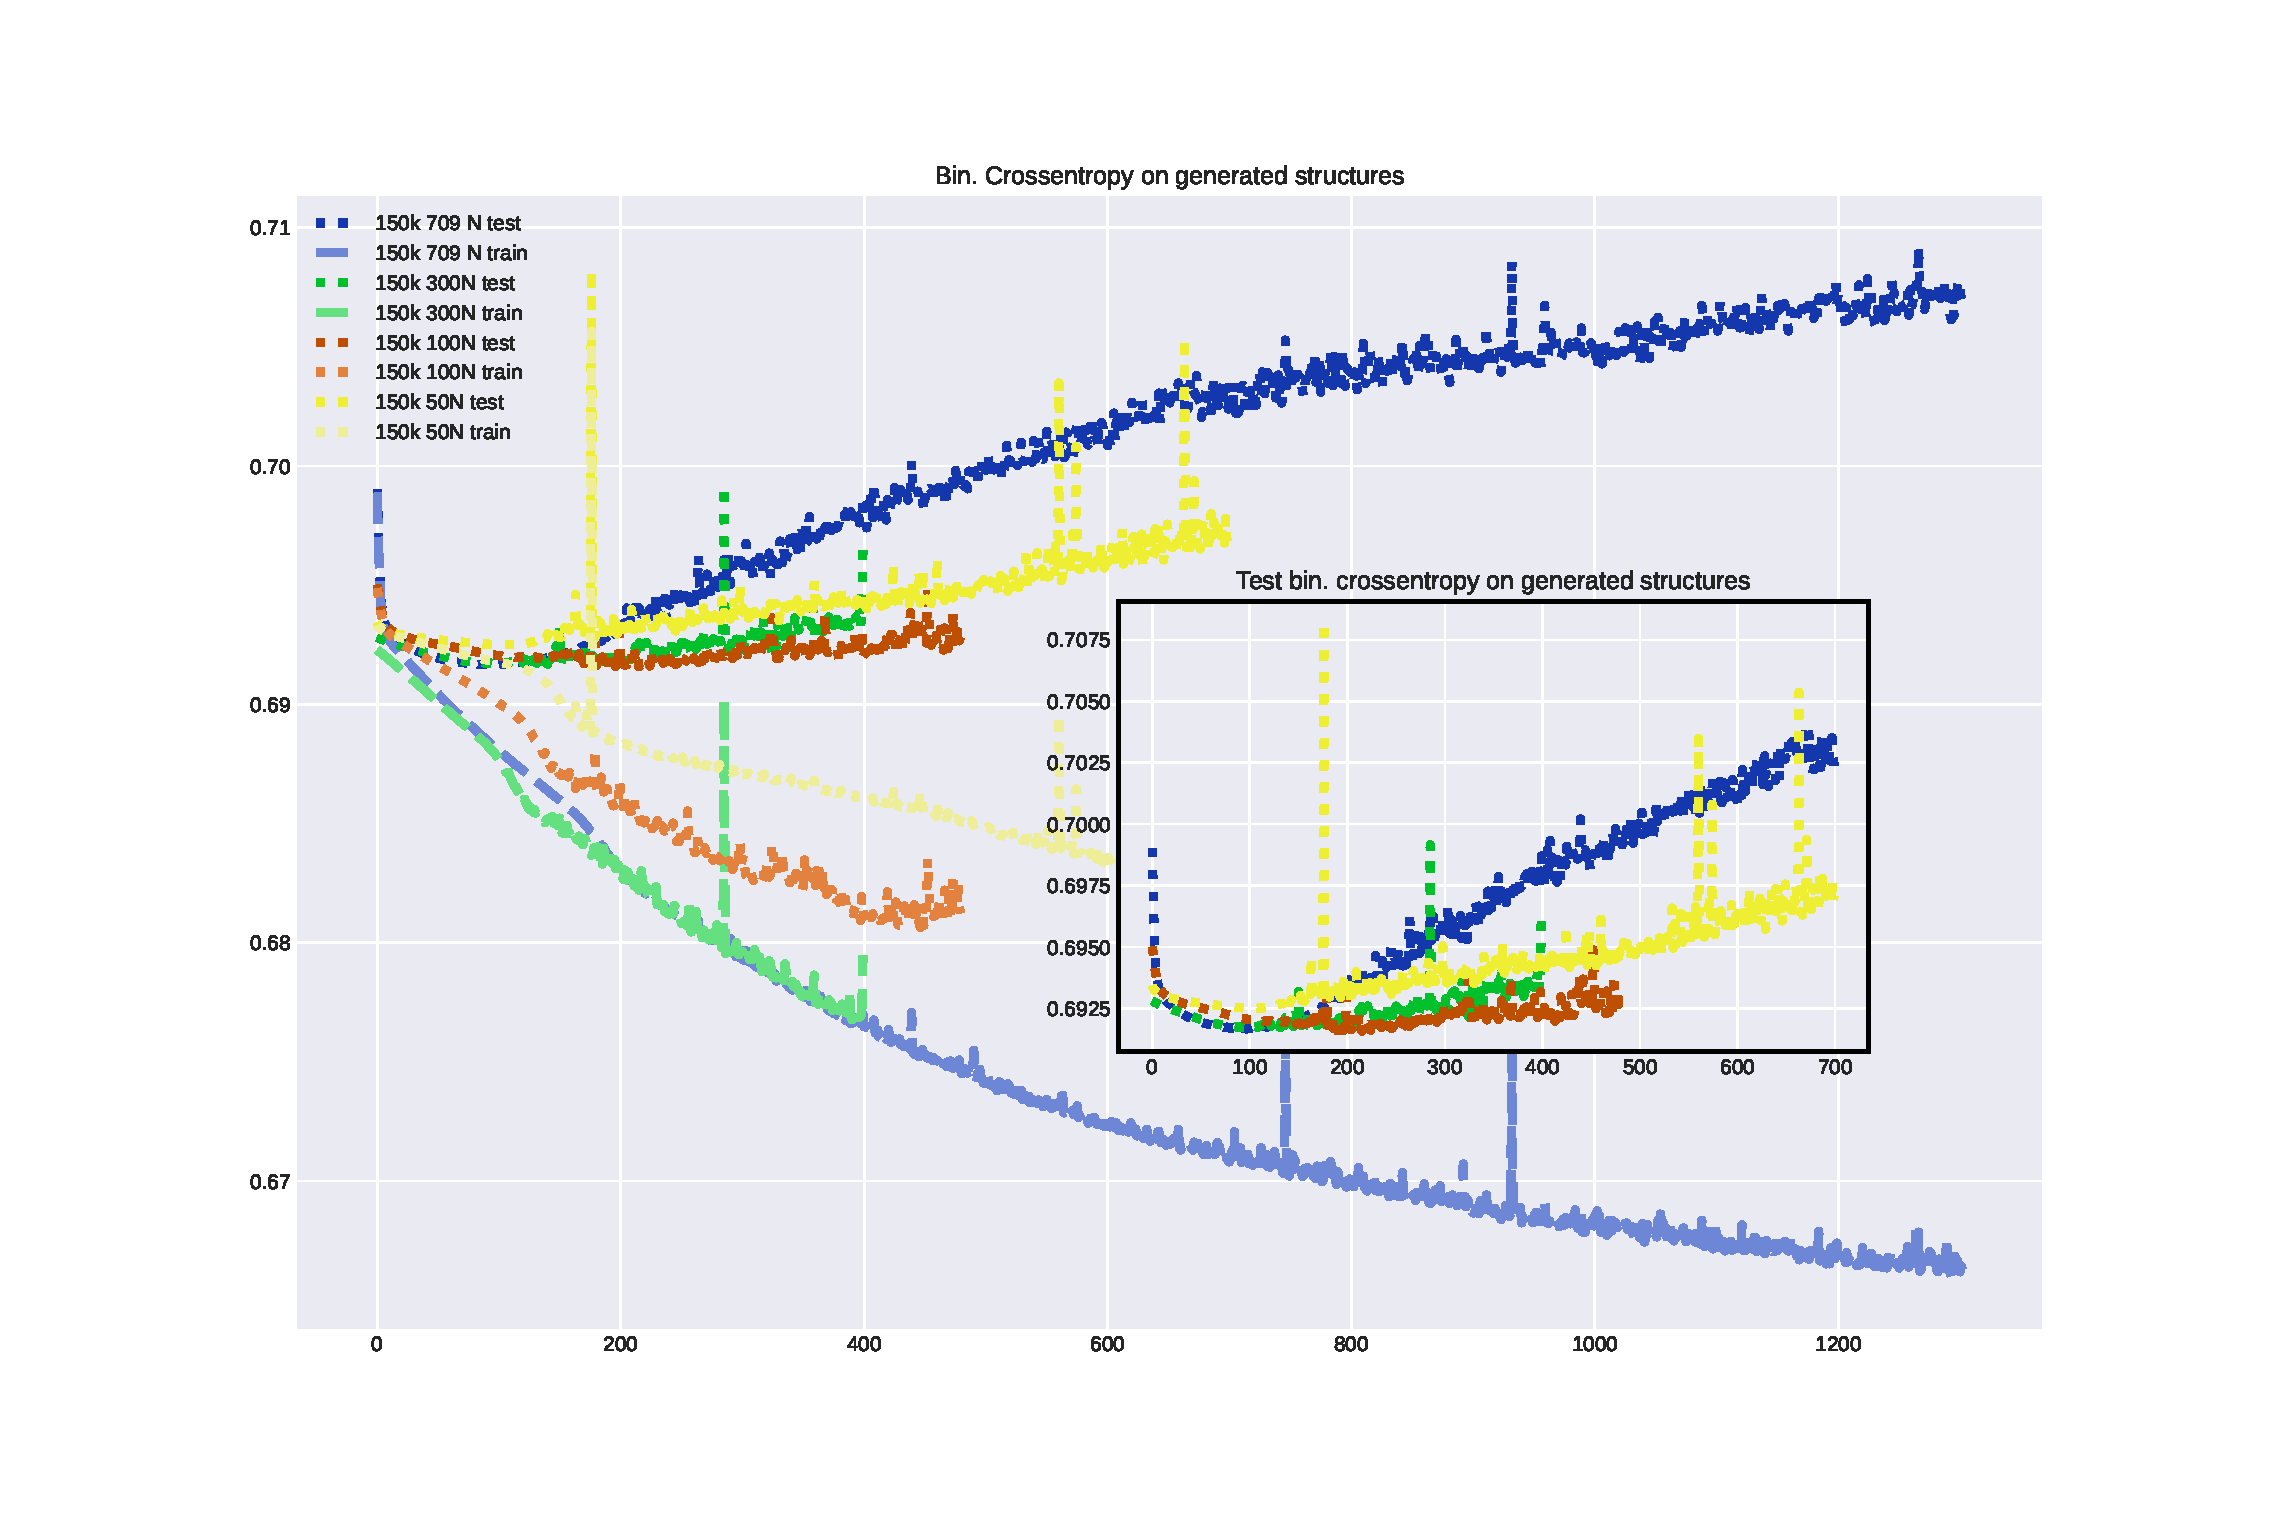
\includegraphics[scale=.500]{imgs/loss-lsize.eps}
\caption{}
\label{}
\end{figure}

\begin{figure}[htp]
\centering
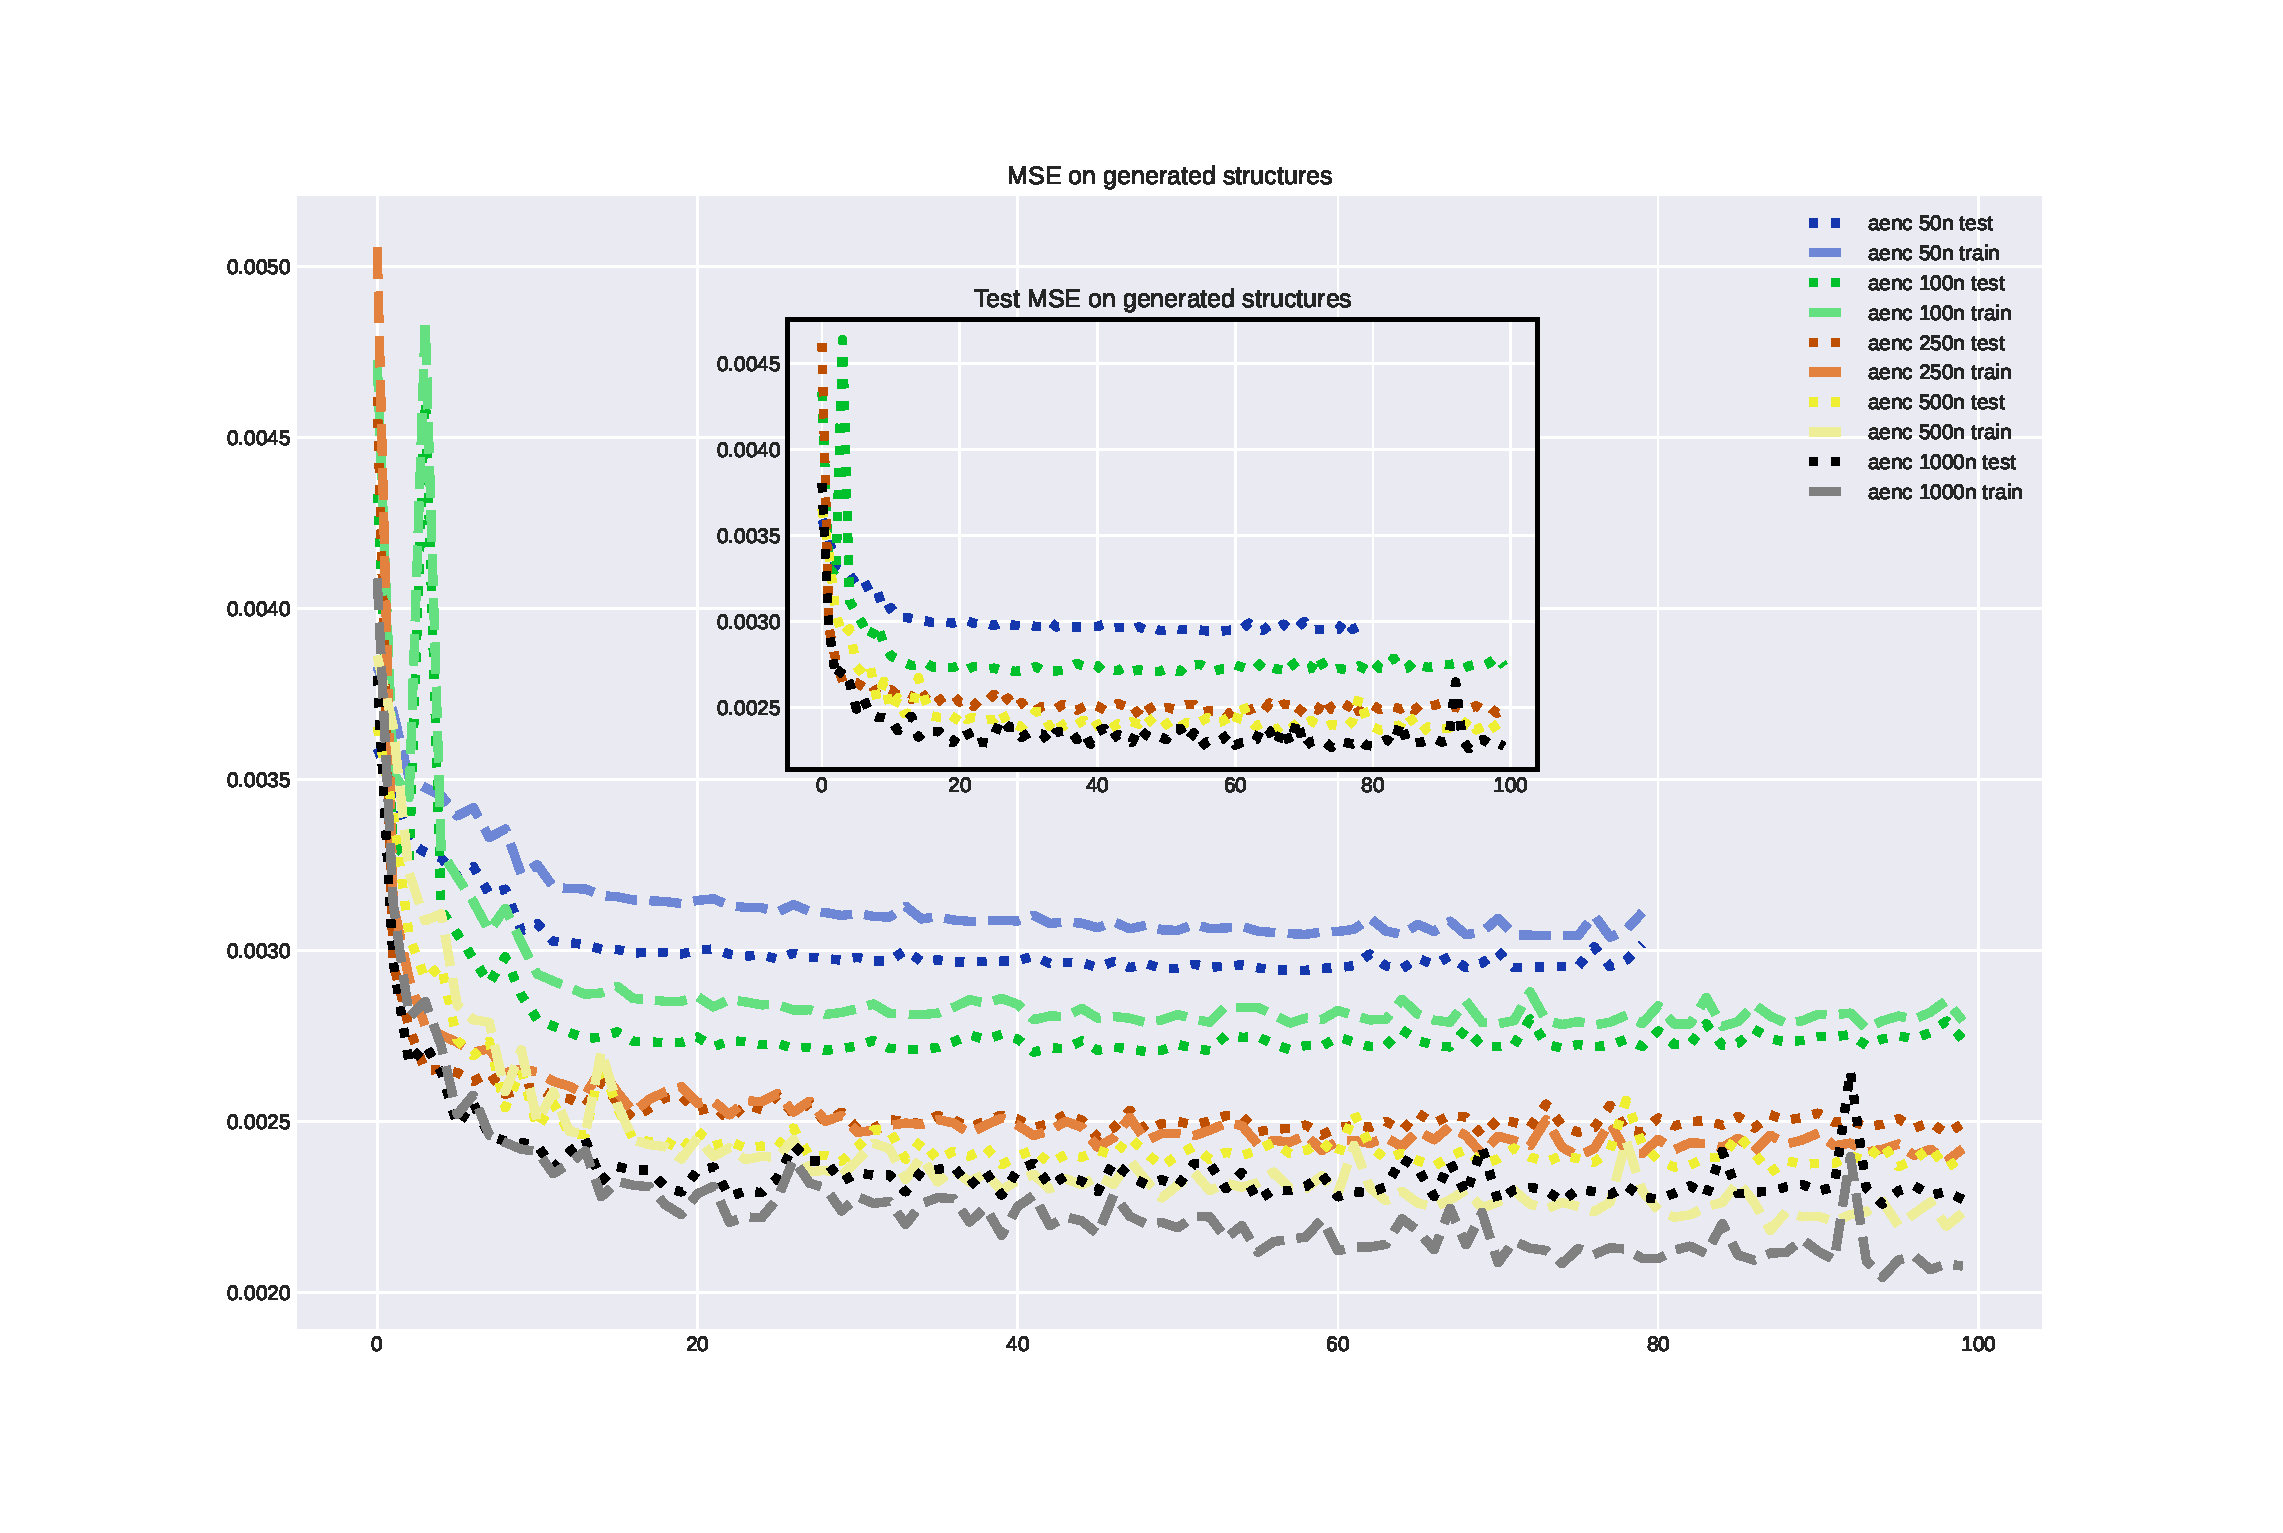
\includegraphics[scale=0.50]{imgs/loss-aenc.eps}
\caption{}
\label{}
\end{figure}

\begin{figure}[htp]
\centering
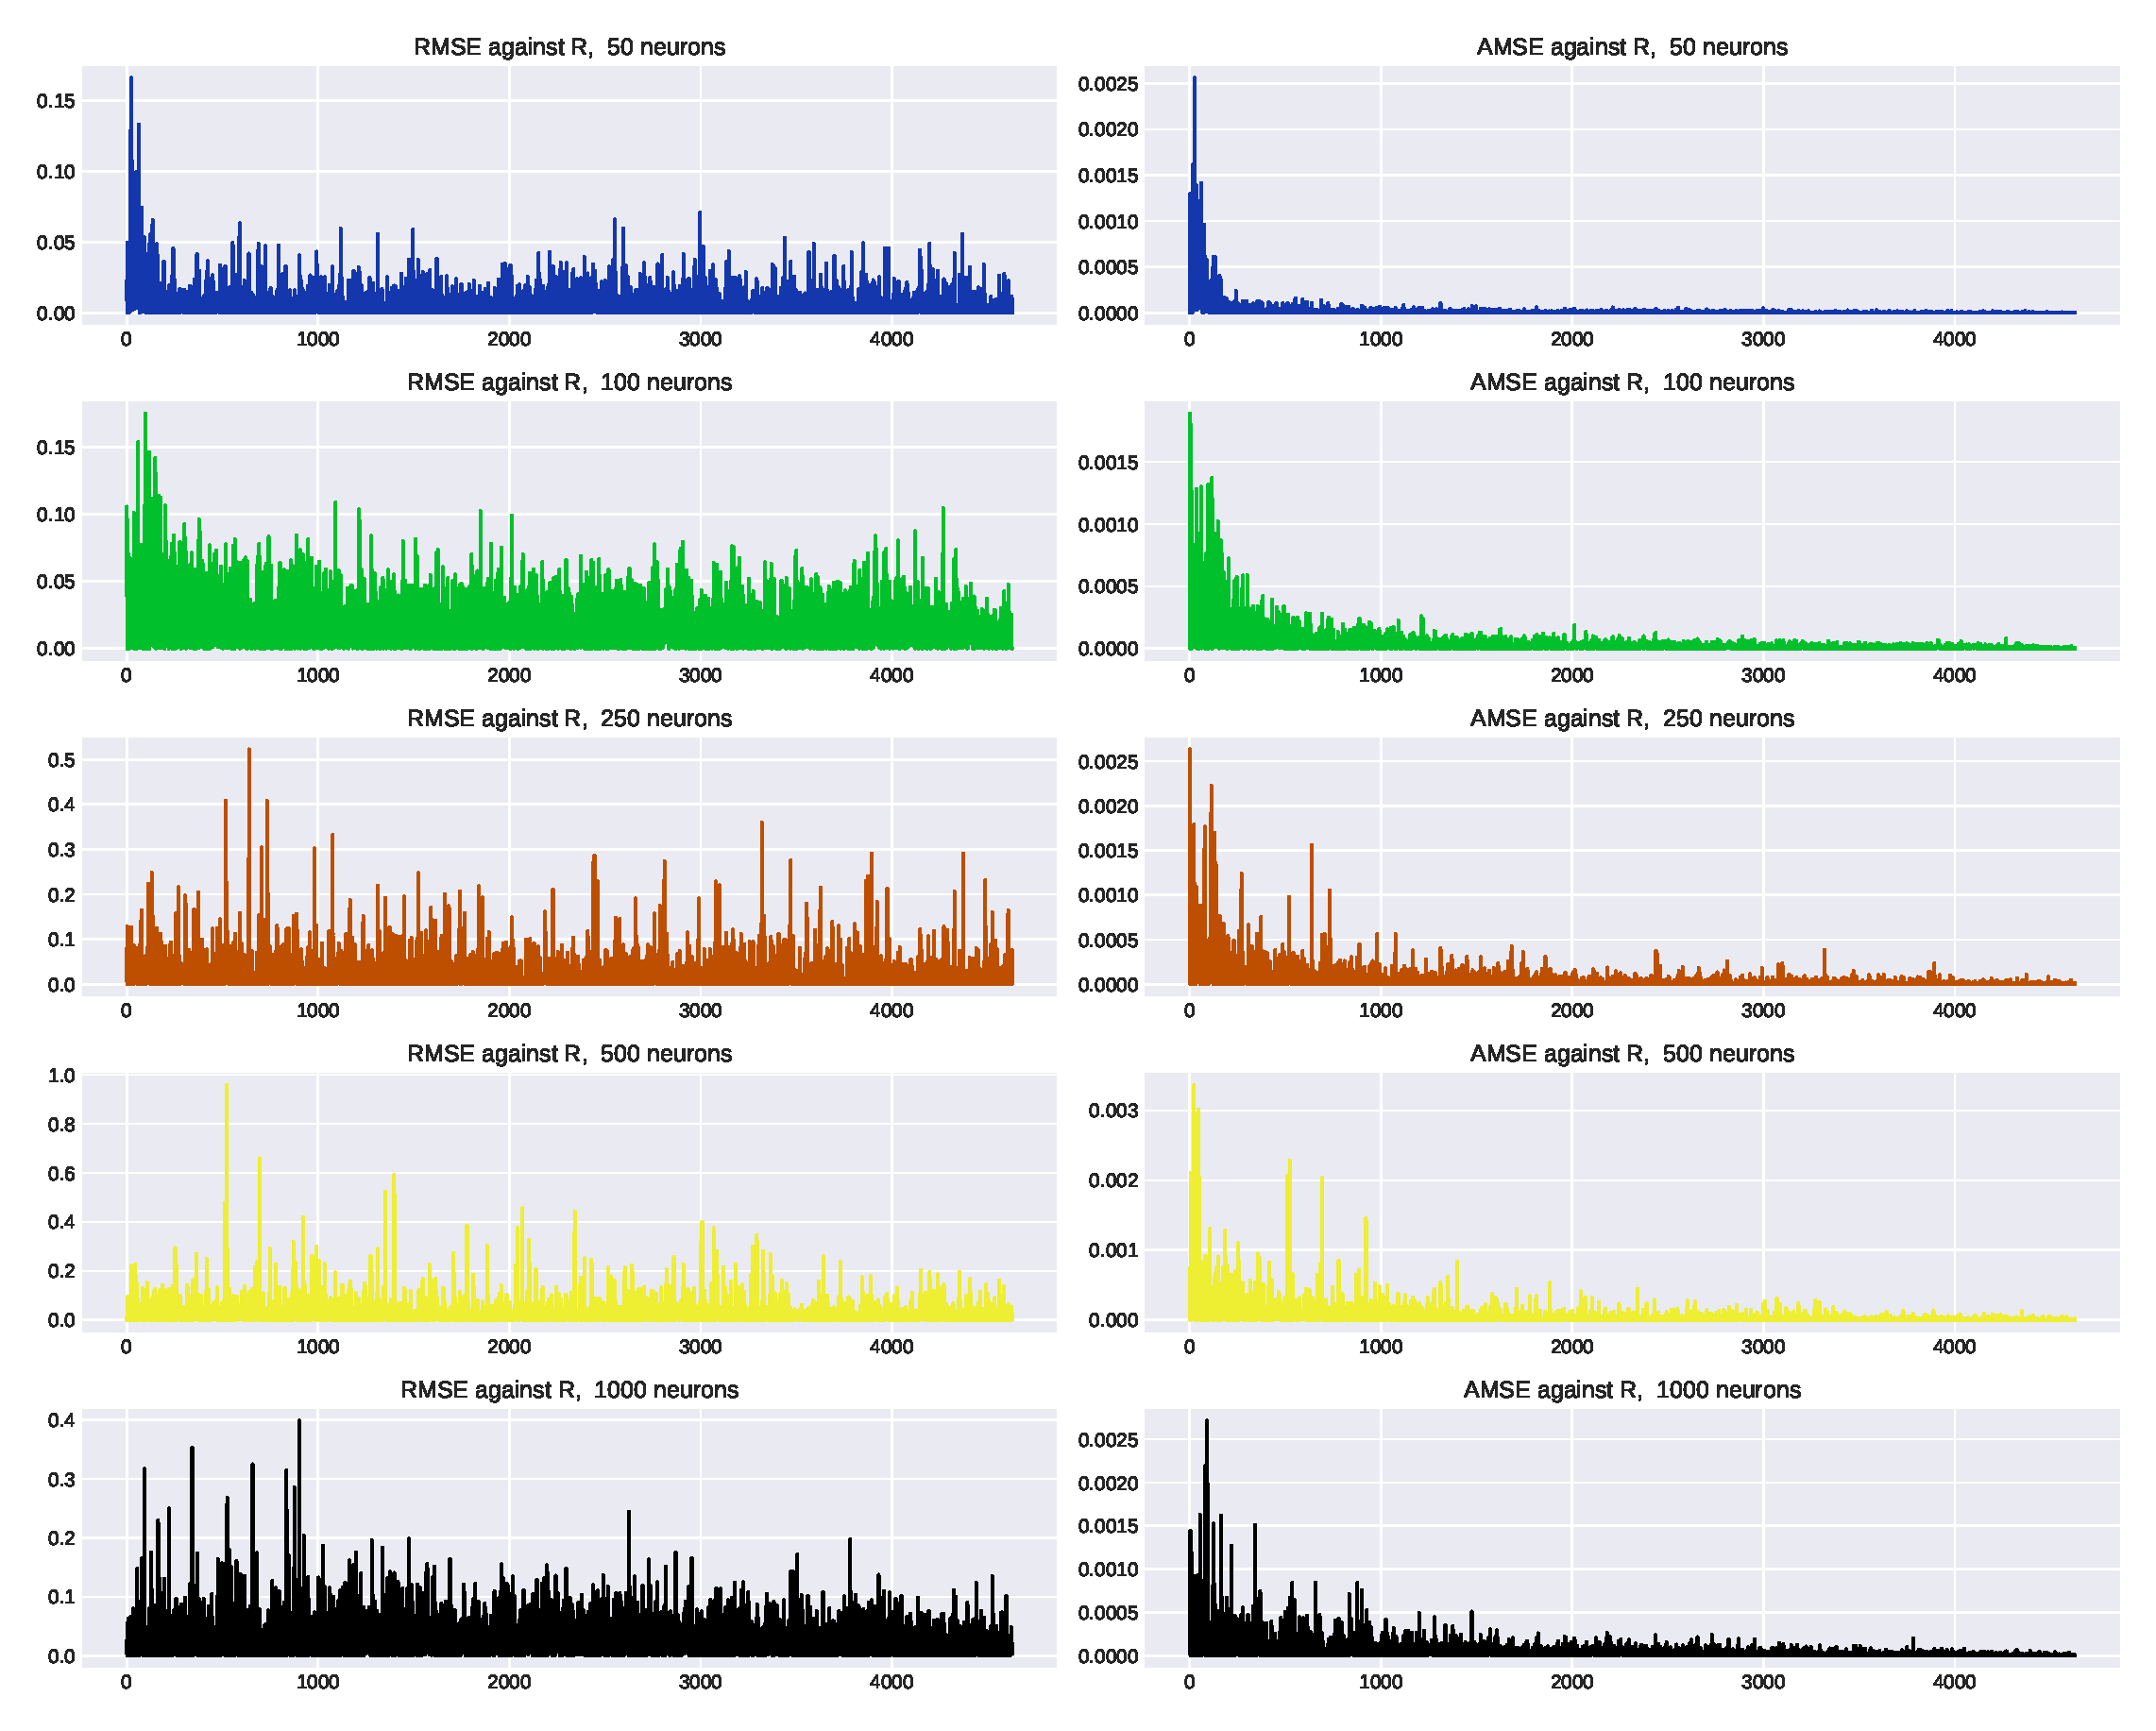
\includegraphics[scale=0.50]{imgs/aenc-errdist.eps}
\caption{}
\label{}
\end{figure}


\begin{figure}[htp]
\centering
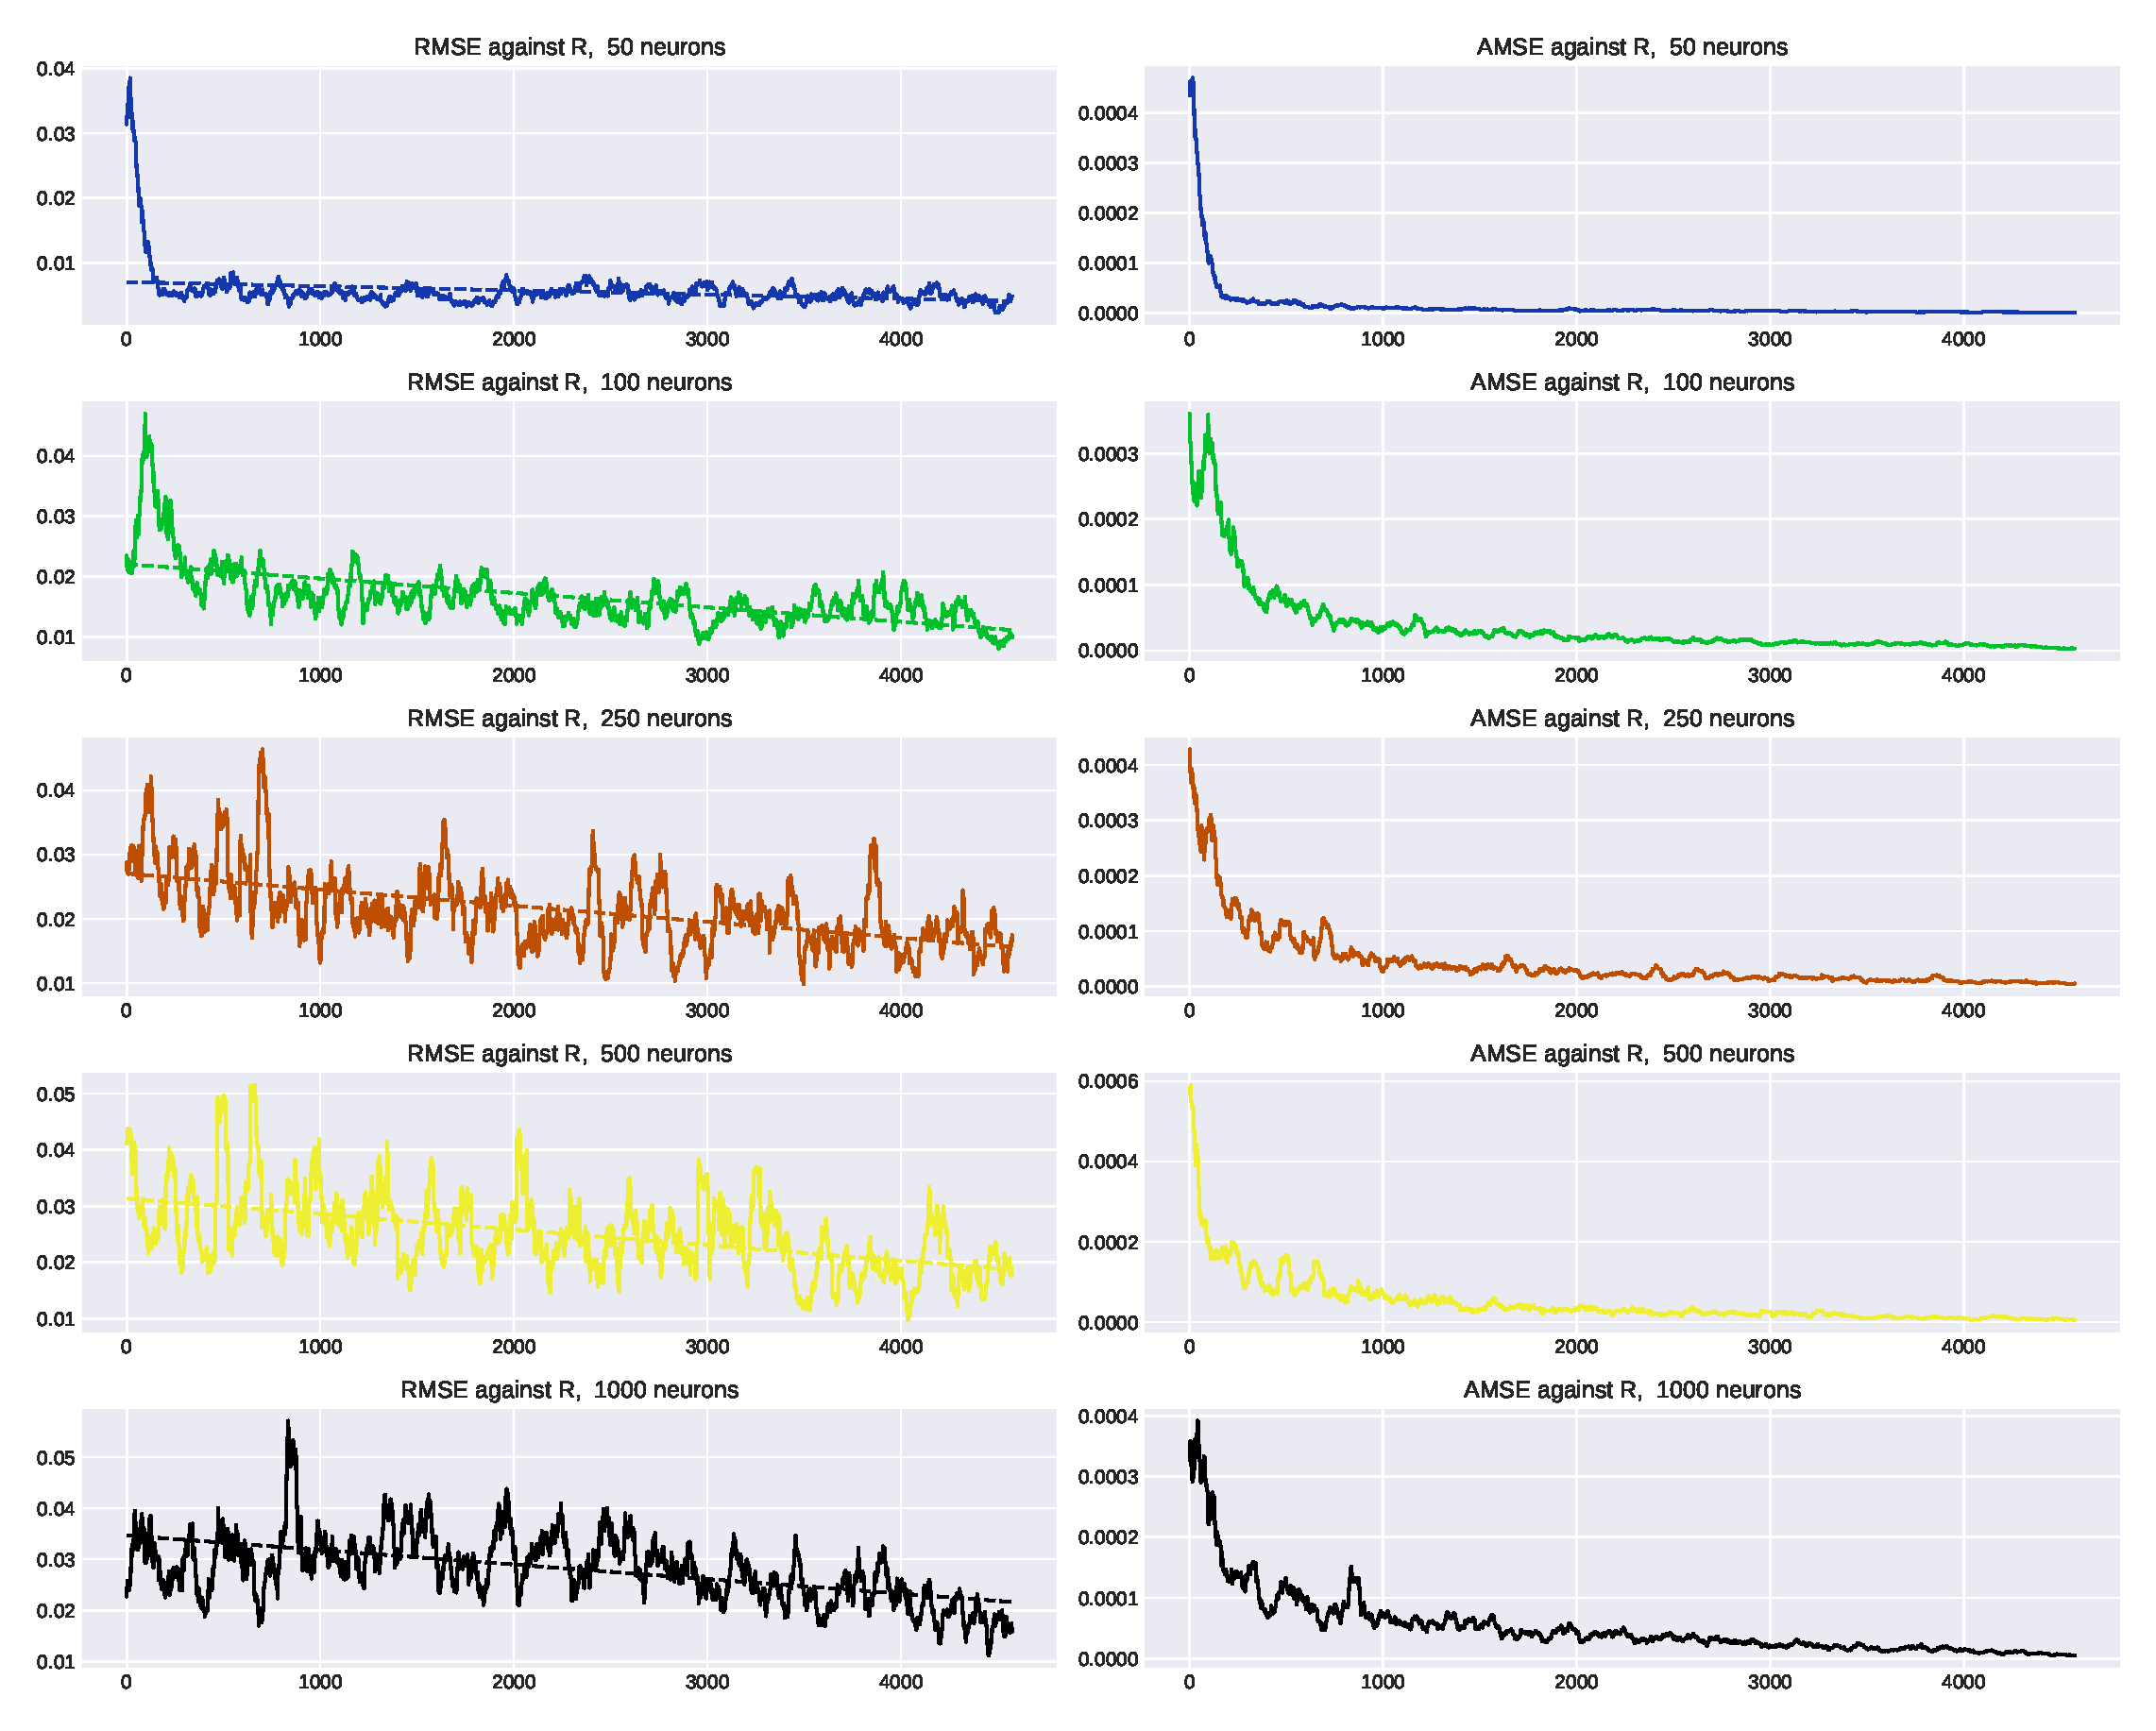
\includegraphics[scale=0.50]{imgs/aenc-errdist_fl.eps}
\caption{}
\label{}
\end{figure}


\newpage
4. модели3 - пробуем автоэнкодеры

Выводы:
пробуем уменьшить запоминающую способность сети, делаем дропауты
Интенсивности не содержать достаточно информации
Добавление параметров
Сделать RFT с phase=0
 
Обучение модели с одним скрытым слоем из 709 нейронов на 709 отражениях из 7000 файлов дало следующие результаты:

TODO 2k, 3, 4k, 10, 1
Сравнить эксп. ошибку с автоэнкодерской
Распеделение ошибок автоэнк/эксп
Сравнить 




\section{РЕЗУЛЬТАТЫ И ВЫВОДЫ}



\end{document}
